%%%%%%%%%%%%%%%%%%%%%%%%%%%%%%%%%%%%%%%%%%%%%%%%%%%%
% Document type, global settings, and packages
%%%%%%%%%%%%%%%%%%%%%%%%%%%%%%%%%%%%%%%%%%%%%%%%%%%%


\documentclass[12pt, oneside, a4paper]{report}   
7
 %12 point font for Times New Roman
\usepackage{graphicx}  %for images and plots
\usepackage[a4paper, left=1.5in, right=1in, top=1in, bottom=1in]{geometry}
\usepackage{setspace}  %use this package to set linespacing as desired
\usepackage{times}  %set Times New Roman as the font
\usepackage[explicit]{titlesec}  %title control and formatting
\usepackage[titles]{tocloft}  %table of contents control and formatting
\usepackage[backend=bibtex, sorting=none, bibstyle=ieee]{biblatex}  %reference manager
\usepackage[bookmarks=true, hidelinks]{hyperref}
\usepackage[page]{appendix}  %for appendices
\usepackage{rotating}  %for rotated, landscape images
\usepackage[normalem]{ulem}  %for italicized text
\usepackage[usenames,dvipsnames]{xcolor}
\definecolor{gold}{rgb}{0.83, 0.69, 0.22}
\definecolor{goldenrod}{rgb}{0.85, 0.65, 0.13}
\usepackage{pdfpages}
\usepackage{listings}
\lstset{breaklines=true}
\lstset{breakatwhitespace=false}
\lstset{literate=::1}
\usepackage{adjustbox}




%%%%%%%%%%%%%%%%%%%%%%
% Start of Document
%%%%%%%%%%%%%%%%%%%%%%

\begin{document}
\doublespacing  %set line spacing
\pagenumbering{gobble}
%%%%%%%%%%%%%%%%%%%%%%%%%%%%%%%%%%%%%
% Title Page
%%%%%%%%%%%%%%%%%%%%%%%%%%%%%%%%%%%%%

\begin{titlepage}

\begin{center}

\vspace{-30mm}

\begin{figure}[h]
    \centering
    
\includegraphics{Others/logo.jpg}
    \label{logo}
\end{figure}

\large Habib University \\
\vspace{5mm}
\textbf{PHY 101L} \\
Mechanic and Thermodynamics Lab\\ 
Fall 2020

\vspace{30mm}
\Large Lab Notebook\\
\large Umme Salma (us04315)\\
\large Munawwar Anwar (ma04289)\\

\end{center}

\clearpage
\thispagestyle{empty}
\null
\clearpage

\end{titlepage}



\pagenumbering{roman}
\setcounter{page}{2} % set the page number appropriately based on the number of 

%%%%%%%%%%%%%%%%%%%%%%%%%%%%%%%%%%%%%
% Table of Contents
%%%%%%%%%%%%%%%%%%%%%%%%%%%%%%%%%%%%%

% Format for Table of Contents
\renewcommand{\cftchapdotsep}{\cftdotsep}  %add dot separators
\renewcommand{\cftchapfont}{\bfseries}  %set title font weight
\renewcommand{\cftchappagefont}{}  %set page number font weight
\renewcommand{\cftchappresnum}{Experiment }
\renewcommand{\cftchapaftersnum}{:}
\renewcommand{\cftchapnumwidth}{6.5em}
\renewcommand{\cftchapafterpnum}{\vskip\baselineskip} %set correct spacing for entries in single space environment
\renewcommand{\cftsecafterpnum}{\vskip\baselineskip}  %set correct spacing for entries in single space environment
\renewcommand{\cftsubsecafterpnum}{\vskip\baselineskip} %set correct spacing for entries in single space environment
\renewcommand{\cftsubsubsecafterpnum}{\vskip\baselineskip} %set correct spacing for entries in single space environment

%format title font size and position (this also applys to list of figures and list of tables)
\titleformat{\chapter}[display]
{\normalfont\bfseries\filcenter}{\chaptertitlename\ \thechapter}{0pt}{\MakeUppercase{#1}}

\renewcommand\contentsname{Table of Contents}
\currentpdfbookmark{Table of Contents}{TOC}
\begin{singlespace}
\tableofcontents
\end{singlespace}



\clearpage

%%%%%%%%%%%%%%%%%%%%%%%%%%%%
%
% Chapters
%
%%%%%%%%%%%%%%%%%%%%%%%%%%%%

%%%%%%%%%%%%%%%%%%%%%%
% formatting
%%%%%%%%%%%%%%%%%%%%%%
% resume page numbering for rest of document
\clearpage
\pagenumbering{arabic}
\setcounter{page}{1} % set the page number appropriately

% Adjust chapter title formatting
\titleformat{\chapter}[display]
{\normalfont\bfseries\filcenter}{Experiment \ \thechapter}{0pt}{\MakeUppercase{#1}}  %spacing between titles
\titlespacing*{\chapter}
  {0pt}{0pt}{30pt}	%controls vertical margins on title
  
% Adjust section title formatting
\titleformat{\section}{\normalfont\bfseries}{\thesection}{1em}{#1}

% Adjust subsection title formatting
\titleformat{\subsection}{\normalfont}{\uline{\thesubsection}}{0em}{\uline{\hspace{1em}#1}}

% Adjust subsubsection title formatting
\titleformat{\subsubsection}{\normalfont\itshape}{\thesubsection}{1em}{#1}

%%%%%%%%%%%%%%%%
% Experiment 1
%%%%%%%%%%%%%%%%

\chapter{Quantifying Uncertainty : Measurement of Gravitational Acceleration}

Date: 5/9/2020

\section{Aim}

In this experiment, our aim is to measure the gravitational acceleration of Earth using a pendulum and quantify various Type A and Type B uncertainties to produce a concrete uncertainty of our measurement. We observe the relationship between the Length of a pendulum and its Time Period. We use a metallic bob with a hook as our pendulum.

\section{Background Theory}

Newton's Law of Gravitation states that `' Any particle of matter in the universe attracts any other with a force varying directly as the product of the masses and inversely as the square of the distance between them. '' Mathematically, it can be expressed as 
$$\vec{F} = -G \frac{m_1 \times m_2}{r^2} \hat{r}$$
where G is the gravitational constant, $m_1$ is the mass of body 1, $m_2$ is the mass of body 2 and $r$ is the separation between the center of masses of both bodies. Newton's second of motion states ``that rate of change of momentum of a body is directly proportional to the force applied'' which can be expressed in the form 
$$ \vec{F} = m \times \vec{a}$$
where m is the mass of the body and a is the acceleration. Combining these both Laws, gives us the following equation
$$ g = -G \frac{M_E}{{R_E}^2} $$
where the $M_E$ is the mass of the Earth and $R_E$ is the radius of the Earth.\\
The length (L) of the pendulum is related to its time period (T) by the following equation:
$$ T = 2\pi\sqrt{\frac{L}{g}} $$
This equation can be re-written by making g the subject :
$$ g = 4\pi^2\frac{L}{T^2} $$

\section{Description of Setup}
% \begin{figure}[h!]
%     \centering
%     \includegraphics[width=\textwidth]{figures/A1.png}
%     \caption{Apparatus}
%     \label{fig:yx}
% \end{figure}
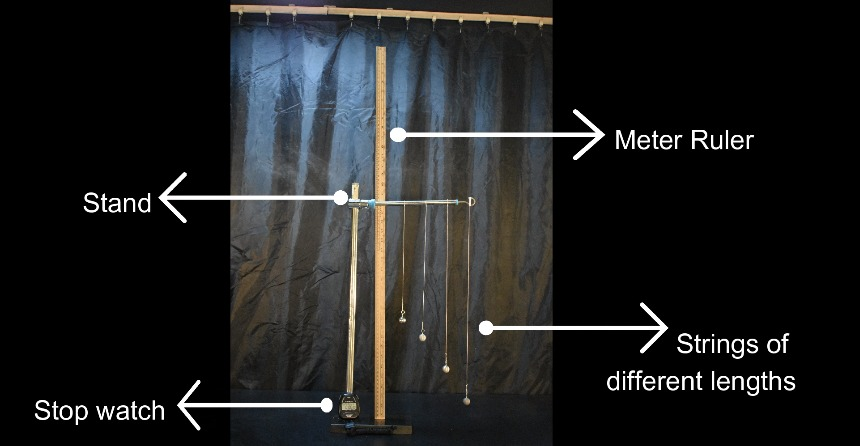
\includegraphics[width=10cm, height=8cm]{figures/fig1g.jpeg} \\
Here the stand with clamp is used to provide a rigid support, metre rule is used to measure the length L of the pendulum , digital stopwatch is used to record the time period of the pendulum and the metallic bob with a hook is used as a pendulum. In this experiment, we use four different length of threads


\section{Method / Procedure}

The length of the thread is measured from the clamp to the center of the metallic bob using the metre Ruler. Digital stopwatch is used to record the time-period for ten oscillations. The same process is repeated 5 times for each  thread. Length of the Pendulum is adjusted by attaching the metallic bob to a thread of different length.Threads of four different lengths are used in this Experiment. \\
The gravitational acceleration $g_i$ is calculated for each different length of pendulum by using the average time period of one oscillation and theory described above. These $g_i$'s are then combined together to calculate the final value of the gravitational acceleration $g$.

\section{Data}

Since the length of the pendulum was only measured it has no type A uncertainty. The type B uncertainty associated with the metre ruler and digital stopwatch are $0.0002m$ and $0.003s$ \\
The lengths of the Pendulum measured using the metre ruler.
\begin{center}
\begin{tabular}{|c|c|c|c|c|c|}
\hline
\textbf{s.No} & \textbf{Height} & \textbf{Upper (cm)} & \textbf{Lower (cm)} & \textbf{Length (cm)} & \textbf{Length (m)} \\ \hline
1             & H1              & 80.7                & 43.0                & 37.7                 & $0.377 \pm 0.0002 $ \\ \hline
2             & H2              & 73.5                & 42.3                & 31.2                 & $0.312 \pm 0.0002 $ \\ \hline
3             & H3              & 68.0                & 42.7                & 25.3                 & $0.253 \pm 0.0002 $ \\ \hline
4             & H4              & 92.7                & 42.0                & 50.7                 & $0.507 \pm 0.0002$ \\ \hline
\end{tabular}
\end{center} 
The time period for ten-oscillations recorded using digital stopwatch.
\begin{center}
\begin{tabular}{|c|c|c|c|c|}
\hline
\textbf{s.No} & \textbf{T\_H1 (s)} & \textbf{T\_H2 (s)} & \textbf{T\_H3 (s)} & \textbf{T\_H4 (s)} \\ \hline
1             & 11.60              & 11.53              & 10.22              & 14.62              \\ \hline
2             & 11.40              & 11.18              & 10.19              & 14.50              \\ \hline
3             & 11.10              & 11.21              & 10.22              & 14.41              \\ \hline
4             & 11.30              & 11.25              & 10.28              & 14.47              \\ \hline
5             & 11.30              & 11.31              & 10.44              & 14.60              \\ \hline
\end{tabular}
\end{center}
Type A uncertainty in the Time Period for each length was calculated using the method mentioned in the MATLAB script . \\
Type A uncertainty in Time Period for H1
\begin{center}
$\sigma_T = 0.0162 s$ \\
$ U_T^A =  0.0081s$ \\
\end{center}
$ U_T = \sqrt{{U_T^A}^2 +{U_T^B}^2}$ \\
$ U_T = \sqrt{0.0081^2+0.003^2}$ \\
$ U_T = 0.0086s $ \\
Total uncertainty in Time Period (T1)  for $H_1$ is $ T = 1.134 \pm 0.009 s$\\
Type A uncertainty in Time Period for H2
\begin{center}
$\sigma_T = 0.0125 s$ \\
$ U_T^A =  0.0062s$ \\
\end{center}
$ U_T = \sqrt{{U_T^A}^2 +{U_T^B}^2}$ \\
$ U_T = \sqrt{0.0062^2+0.003^2}$ \\
$ U_T = 0.0069s $ \\
Total uncertainty in Time Period (T2)  for $H_2$ is $ T = 1.130 \pm 0.007 s$\\
Type A uncertainty in Time Period for H3
\begin{center}
$\sigma_T = 0.090 s$ \\
$ U_T^A =  0.0045s$ \\
\end{center}
$ U_T = \sqrt{{U_T^A}^2 +{U_T^B}^2}$ \\
$ U_T = \sqrt{0.0045^2+0.003^2}$ \\
$ U_T = 0.0053s $ \\
Total uncertainty in Time Period (T3) for $H_3$ is $ T = 1.027 \pm 0.005 s$\\
Type A uncertainty in Time Period for H4
\begin{center}
$\sigma_T = 0.079 s$ \\
$ U_T^A =  0.0040s$ \\
\end{center}
$ U_T = \sqrt{{U_T^A}^2 +{U_T^B}^2}$ \\
$ U_T = \sqrt{0.0040^2+0.003^2}$ \\
$ U_T = 0.0049s $ \\
Total uncertainty in Time Period (T4)  for $H_4$ is $ T = 1.452 \pm 0.005 s$
    
\section{Data Analysis}
The formula for calculating g is as follows :
$$ g = 4\pi^2\frac{L}{T^2} $$
Transferring the uncertainty in Time and Length to gravitational acceleration
$$ U_g = \sqrt{\Bigg({4\pi^2 \frac{(-2)L}{T^3} \Delta T}\Bigg)^2+\Bigg({4\pi^2 \frac{1}{T^2} \Delta L}\Bigg)^2}$$
$$ U_g = \frac{4\pi^2}{T^2} L \sqrt{ {\bigg( \frac{-2 \Delta T}{T}  \bigg)}^2    +  {\bigg( \frac{\Delta L}{L} \bigg)}^2} $$

$$ U_g = g\sqrt{ {\bigg( \frac{-2 \Delta T}{T}  \bigg)}^2    +  {\bigg( \frac{\Delta L}{L} \bigg)}^2} $$
Calculating g1 
$$ g_1 = 4\pi^2 \frac{L_1}{{T1}^2} = 4\pi^2 \frac{0.377}{{1.134}^2}  = 11.5738  m/s^2 $$ 
$$ \sigma_1 = 11.5738 \sqrt{{\bigg(\frac{-2 \times 0.009}{1.134}\bigg)}^2+{\bigg(\frac{0.0002}{0.377}\bigg)}^2} = 0.1761  m/s^2 $$
$$ g = 11.5738 \pm 0.1761 m/s^2 $$
Calculating g2
$$ g_2 = 4\pi^2\frac{L_2}{{T2}^2} = 4\pi^2 \frac{0.312}{1.130^2}  = 9.6531  m/s^2  $$ 
$$ \sigma_2 = 9.6531 \sqrt{{\bigg(\frac{-2 \times 0.007}{1.130}  \bigg)}^2+{\bigg( \frac{0.0002}{0.312} \bigg)}^2} = 0.1155 m/s^2 $$
$$ g = 9.6531 \pm 0.1155 m/s^2$$
Calculating g3
$$ g_3 = 4\pi^2\frac{L_1}{{T1}^2} = 4\pi^2 \frac{0.253}{{1.027}^2}  = 9.4698 m/s^2$$ 
$$ \sigma_3 = 9.4698 \sqrt{{\bigg( \frac{-2 \times 0.005}{1.027} \bigg)}^2+{\bigg( \frac{0.0002}{0.253} \bigg)}^2} = 0.0988  m/s^2 $$
$$ g = 9.4698 \pm 0.0988 m/s^2 $$
Calculating g4
$$ g_4 = 4\pi^2\frac{L_1}{{T1}^2} = 4\pi^2 \frac{0.5070}{1.452^2}  = 9.4937  m/s^2 $$ 
$$ \sigma_4 = 9.4937 \sqrt{ {\bigg( \frac{-2 \times 0.005}{1.452}  \bigg)}^2    +  {\bigg( \frac{0.0002}{0.5070} \bigg)}^2} = 0.0642 m/s^2$$
$$ g = 9.4937 \pm 0.0642 m/s^2$$
Now we can combine the $g1,g2,g3$ and $g4$ and their uncertainties to obtain the final value for gravitational acceleration and its uncertainty.

$$ g = \frac{ (\frac{g_1}{{\sigma_1}^2}+\frac{g_2}{{\sigma_2}^2}+\cdots)} {(\frac{1}{{\sigma_1}^2}+\frac{1}{{\sigma_2}^2}+\cdots)} = \frac{\sum_{i} \frac{g_i}{{\sigma_i}^2} }{\sum_{i} \frac{1}{{\sigma_i}^2} }$$
Combining the uncertainties in $g1,g2,g3$ and $g4$
$$ \sigma^2 =  \frac{1}{\sum_{i} \frac{1}{{\sigma_i}^2} }$$

$$ g = 9.6631  \pm 0.0472 m/s^2$$





\section{Discussion \& Conclusion}

The percentage uncertainty is 0.98 \%, and standard value of gravitational acceleration is not in the range $ g = 9.6631  \pm 0.0472 m/s^2$. Possible factors of uncertainty and errors are external factors such as wind and human errors in recording final time. Therefore there is a chance that hypothesis is not valid since standard value is not in the range. Perhaps a more accurate set up could have given results that would agree with hypothesis. Improvement can be a more accurate mechanism for recording time such as light gate, we can also ensure that external factors such as wind are minimized by using wind blockers and we can also use a fiducial marker to mark the mean of an oscillation. 

% Summarize and discuss the experimental results, what do the results say about your hypothesis, if such a hypothesis was made for the experiment. Mention the uncertainty in the calculated quantity Be precise and only include scientific discussion.


\section{MATLAB Script}
\lstinputlisting{matlabCodes/Experiment1.m}





%%%%%%%%%%%%%%%
%Experiment 2
%%%%%%%%%%%%%%%

% \chapter{Title of the Experiment}


=-\chapter{Equivalent spring constant of combination of springs}

Date: 14/9/2020

% Date: 5/9/2020

\section{Aim}

In this experiment, our aim is to calculate the equivalent spring constant of combination of springs, in both series and parallel. We derive the relationship of spring constant by applying varying weight on springs in series and parallel.


\section{Background Theory}

Hooke's Law states force applied on a spring is proportional to its extension, given its limit of proportionality has not reached. Mathematically, it can be expressed as $$ F= k \Delta x $$ where F is force applied, k denotes spring constant and $\Delta x$ is change in length of spring. When the spring reaches its elastic limit then it can not return back to its original shape and is deformed. 
When the springs are attached in series, the extension is equal to
    $$ \Delta x = \Delta x_1 + \Delta x_2 $$
The force that is applied  on both the strings is same, consequently :
    $$ F = k(\Delta x_1 + \Delta x_2) $$
    $$ F = k_1 \Delta x_1 $$
    $$ F = k_2 \Delta x_2 $$
We can then combine these equations to get an expression for k, there combined spring constant.
    $$ k_1 \Delta x_1 =  k_2 \Delta x_2 $$
    $$ \Delta x_2 = \frac{K_1 \Delta x_1}{k_2} $$
    $$ F = k(\Delta x_1 + \frac{K_1 \Delta x_1}{k_2}) $$ 
    $$ F = k(1 + \frac{k1}{k2}) \Delta x_1 $$
    $$ k_1 \Delta x_1 = k(1 + \frac{k1}{k2}) \Delta x_1 $$
    $$ k = \frac{k_1 \times k_2}{k_1 +k_2} $$
When springs are attached in parallel, the total force is equal to
    $$ F = F_1 + F_2 $$
The extension of both the springs is same, Consequently:
    $$ F = k \Delta x $$
    $$ F_1 = k_1 \Delta x $$
    $$ F_2 = k_2 \Delta x $$
We can then combine these equations to get an expression for k,
there combined spring constant.

$$ k \Delta x = k_1 \Delta x + k_2 \Delta x $$
$$ k \Delta x = \Delta x( k_1 + k_2) $$
$$ k = k_1 + k_2 $$




% \begin{figure}[htbp]
% \centerline{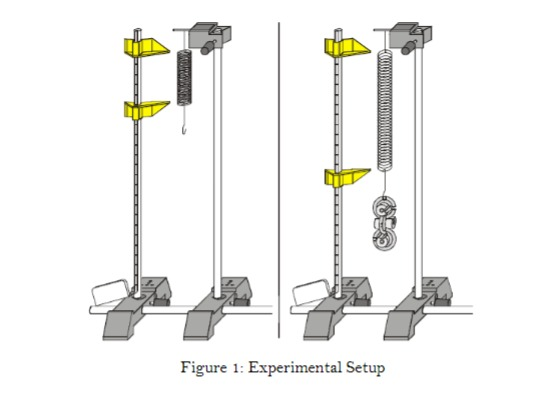
\includegraphics[width=3in, height=2in]{figures/fig3.jpeg}}
% \caption{This is an image from a text that uses color to teach music.}
% % \label{fig}
% \end{figure}

% \begin{figure}[h!]
%     \centering
%     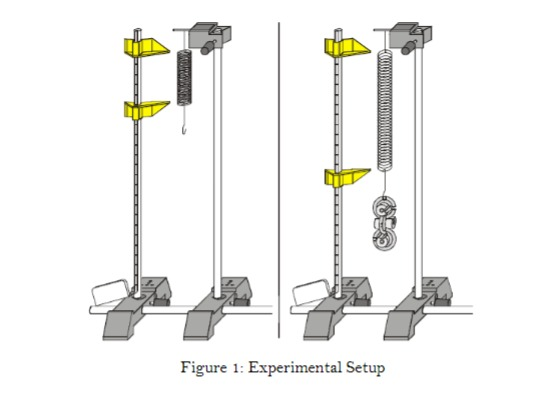
\includegraphics[width=\textwidth]{figures/fig3.jpeg}
%     \caption{Apparatus}
%     \label{fig:yx}
% \end{figure}
\section{Description of Setup}
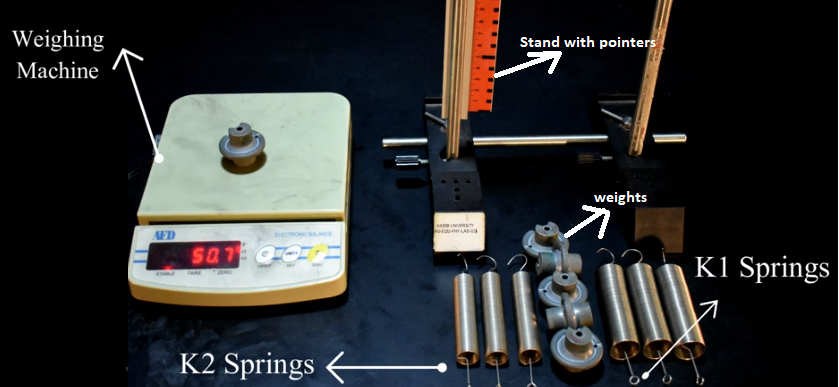
\includegraphics[width=12cm, height=7cm]{figures/fig1.png} \\
Here the stand with pointers gives easy access to measuring the length and spring is supported on a clamp.The weights are then suspended from the spring.

\section{Method / Procedure}
The initial length of the spring is measured using the pointer stand and weights are suspended and the springs length is measured. This is repeated with adding more weights and change in the length of spring is measured. 
This is carried out for setting up the springs in series and parallel. 
The springs constant is calculated using Hooke's law by determining slope of the graph of extension against weight of masses.

\section{Data}

In this experiment, since the mass of the weights and the extension in length is measured only once they don't not have type A uncertainty. The type B certainty associated with the length and mass is respectively 0.0002m and 0.03g

\begin{center}
    
\begin{tabular}{|c|c|c|c|c|}
\hline
\multicolumn{5}{|c|}{\textbf{Initial Measurements}}                     \\ \hline
Springs & dia   (cm) & single   (cm) & series   (cm) & parallel   (cm) \\ \hline
K1      & 2.051      & 7.7           & 22.9          & 7.7             \\ \hline
K2      & 1.524      & 7.7           & 20.3          & 7.7             \\ \hline
K1+K2   & -          & -             & 21.9          & 7.7             \\ \hline
\end{tabular}
\end{center}

\begin{center}
\begin{tabular}{|c|c|c|c|c|c|}
\hline
\multicolumn{6}{|c|}{\textbf{K1 (single)}}                                          \\ \hline
s.No & Mass   (grams) & Upper   (cm) & Lower   (cm) & Diff     (cm) & Ext      (cm) \\ \hline
1    & 0              & 94.2         & 86.5         & 7.7           & 0             \\ \hline
2    & 50.7           & 94.2         & 81.9         & 12.3          & 4.6           \\ \hline
3    & 101.4          & 94.2         & 77.2         & 17            & 9.3           \\ \hline
4    & 152.1          & 94.2         & 72.7         & 21.5          & 13.8          \\ \hline
5    & 202.8          & 94.2         & 68.1         & 26.1          & 18.4          \\ \hline
6    & 253.5          & 94.2         & 63.6         & 30.6          & 22.9          \\ \hline
7    & 304.2          & 94.2         & 58.3         & 35.9          & 28.2          \\ \hline
\end{tabular}
\end{center}

\begin{center}
\begin{tabular}{|c|c|c|c|c|c|}
\hline
\multicolumn{6}{|c|}{\textbf{K1 (series)}}                                          \\ \hline
s.No & Mass   (grams) & Upper   (cm) & Lower   (cm) & Diff     (cm) & Ext      (cm) \\ \hline
1    & 0              & 94.2         & 71.3         & 22.9          & 0             \\ \hline
2    & 50.7           & 94.2         & 62.6         & 31.6          & 8.7           \\ \hline
3    & 101.4          & 94.2         & 53.1         & 41.1          & 18.2          \\ \hline
4    & 152.1          & 94.2         & 43.6         & 50.6          & 27.7          \\ \hline
5    & 202.8          & 94.2         & 34.2         & 60            & 37.1          \\ \hline
6    & 253.5          & 94.2         & 25           & 69.2          & 46.3          \\ \hline
7    & 304.2          & 94.2         & 15.7         & 78.5          & 55.6          \\ \hline
\end{tabular}
\end{center}

\begin{center}
\begin{tabular}{|c|c|c|c|c|c|}
\hline
\multicolumn{6}{|c|}{\textbf{K1 (parallel)}}                                        \\ \hline
s.No & Mass   (grams) & Upper   (cm) & Lower   (cm) & Diff     (cm) & Ext      (cm) \\ \hline
1    & 0              & 94.2         & 86.5         & 7.7           & 0             \\ \hline
2    & 50.7           & 94.2         & 84           & 10.2          & 2.5           \\ \hline
3    & 101.4          & 94.2         & 81.7         & 12.5          & 4.8           \\ \hline
4    & 152.1          & 94.2         & 79.2         & 15            & 7.3           \\ \hline
5    & 202.8          & 94.2         & 77.2         & 17            & 9.3           \\ \hline
6    & 253.5          & 94.2         & 74.7         & 19.5          & 11.8          \\ \hline
7    & 304.2          & 94.2         & 72.3         & 21.9          & 14.2          \\ \hline
\end{tabular}
\end{center}

\begin{center}
\begin{tabular}{|c|c|c|c|c|c|}
\hline
\multicolumn{6}{|c|}{\textbf{K2 (single)}}                  \\ \hline
s.No & Mass   (grams) & l1   & l2   & final & Ext      (cm) \\ \hline
1    & 0              & 94.2 & 86.5 & 7.7   & 0             \\ \hline
2    & 50.7           & 94.2 & 84.9 & 9.3   & 1.6           \\ \hline
3    & 101.4          & 94.2 & 82.8 & 11.4  & 3.7           \\ \hline
4    & 152.1          & 94.2 & 81   & 13.2  & 5.5           \\ \hline
5    & 202.8          & 94.2 & 79.1 & 15.1  & 7.4           \\ \hline
6    & 253.5          & 94.2 & 77.4 & 16.8  & 9.1           \\ \hline
7    & 304.2          & 94.2 & 75.6 & 18.6  & 10.9          \\ \hline
\end{tabular}
\end{center}

\begin{center}
    
\begin{tabular}{|c|c|c|c|c|c|}
\hline
\multicolumn{6}{|c|}{\textbf{K1 and K2 (series)}}                                   \\ \hline
s.No & Mass   (grams) & Upper   (cm) & Lower   (cm) & Diff     (cm) & Ext      (cm) \\ \hline
1    & 0              & 94.2         & 72.3         & 21.9          & 0             \\ \hline
2    & 50.7           & 94.2         & 65.8         & 28.4          & 6.5           \\ \hline
3    & 101.4          & 94.2         & 59.4         & 34.8          & 12.9          \\ \hline
4    & 152.1          & 94.2         & 52.5         & 41.7          & 19.8          \\ \hline
5    & 202.8          & 94.2         & 46.2         & 48            & 26.1          \\ \hline
6    & 253.5          & 94.2         & 39.5         & 54.7          & 32.8          \\ \hline
7    & 304.2          & 94.2         & 33           & 61.2          & 39.3          \\ \hline
\end{tabular}
\end{center}


\begin{center}
\begin{tabular}{|c|c|c|c|c|c|}
\hline
\multicolumn{6}{|c|}{\textbf{K1 and K2 (series)}}                                   \\ \hline
s.No & Mass   (grams) & Upper   (cm) & Lower   (cm) & Diff     (cm) & Ext      (cm) \\ \hline
1    & 0              & 94.2         & 72.3         & 21.9          & 0             \\ \hline
2    & 50.7           & 94.2         & 65.8         & 28.4          & 6.5           \\ \hline
3    & 101.4          & 94.2         & 59.4         & 34.8          & 12.9          \\ \hline
4    & 152.1          & 94.2         & 52.5         & 41.7          & 19.8          \\ \hline
5    & 202.8          & 94.2         & 46.2         & 48            & 26.1          \\ \hline
6    & 253.5          & 94.2         & 39.5         & 54.7          & 32.8          \\ \hline
7    & 304.2          & 94.2         & 33           & 61.2          & 39.3          \\ \hline
\end{tabular}
\end{center}


\section{Data Analysis}
\begin{center}
\begin{figure}[h!]
    \centering
    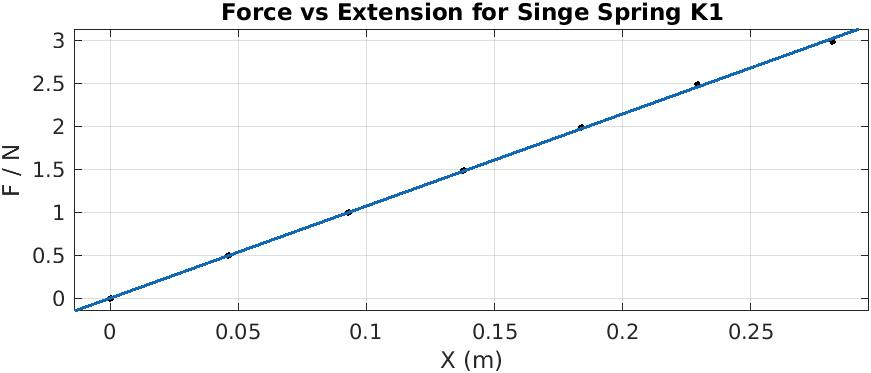
\includegraphics[width=\textwidth]{figures/K1.jpg}
    \caption{Graph of Force vs Extension for spring K1}
    \label{fig:k1}
\end{figure}
\end{center}


$$ K1_{single} = 10.72 N/m $$

\newpage
\begin{center}
\begin{figure}[h!]
    \centering
    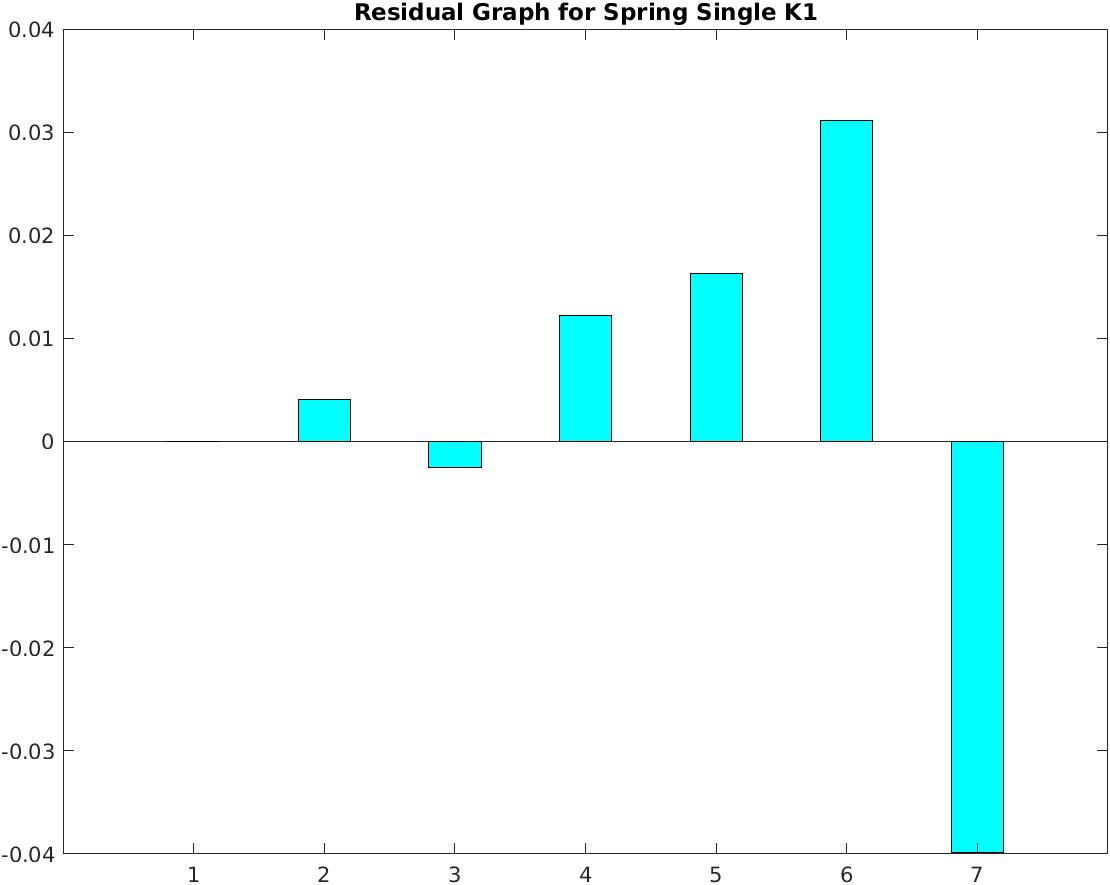
\includegraphics[width=\textwidth]{figures/K1_S_R.jpg}
    \caption{Residual Plot for Single Spring K1}
    \label{fig:k1_S_R}
\end{figure}
\end{center}

\begin{center}
\begin{figure}[h!]
    \centering
    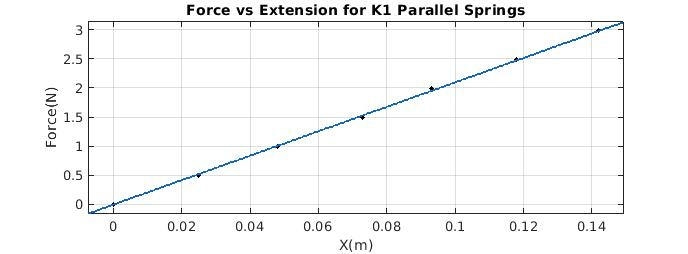
\includegraphics[width=\textwidth]{figures/K1_P.jpg}
    \caption{Graph of Force vs Extension for K1 Parallel Springs}
    \label{fig:k1_P}
\end{figure}
\end{center}
$$ K1_{Parallel} = 21 N/m $$
\newpage
\begin{center}
\begin{figure}[h!]
    \centering
    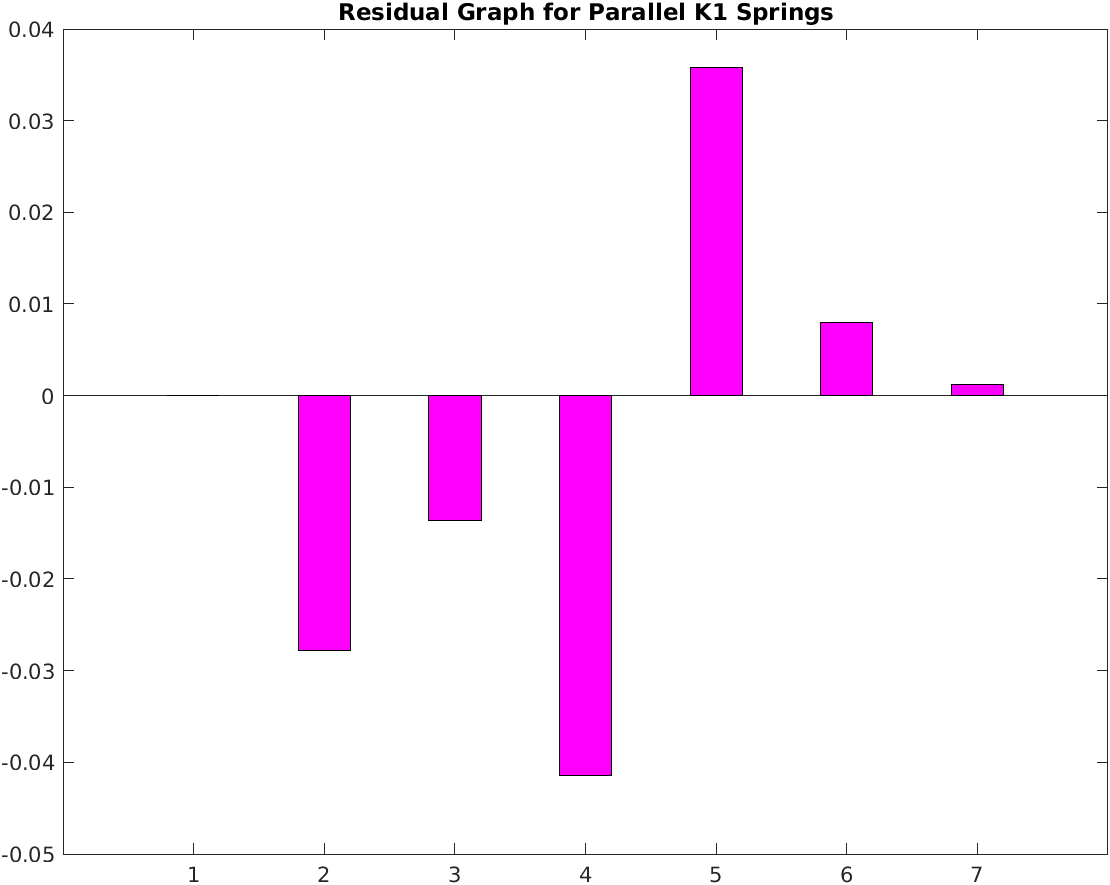
\includegraphics[width=\textwidth]{figures/K1_P_R.png}
    \caption{Residual Plot for Single K1 Parallel Springs}
    \label{fig:k1_P_R}
\end{figure}
\end{center}

\begin{center}
\begin{figure}[h!]
    \centering
    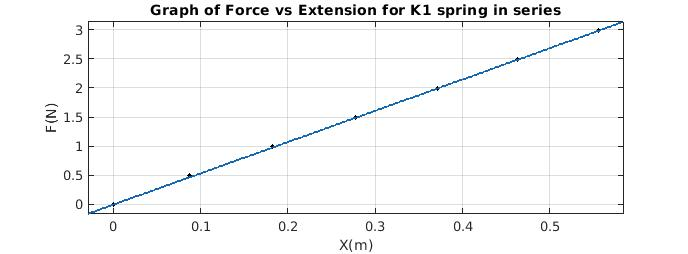
\includegraphics[width=\textwidth]{figures/K1_S_se.jpg}
    \caption{Graph of Force vs Extension for K1 Springs in Series}
    \label{fig:k1_S_se}
\end{figure}
\end{center}
$$ K1_{Parallel} = 5.375 N/m $$
\newpage
\begin{center}
\begin{figure}[h!]
    \centering
    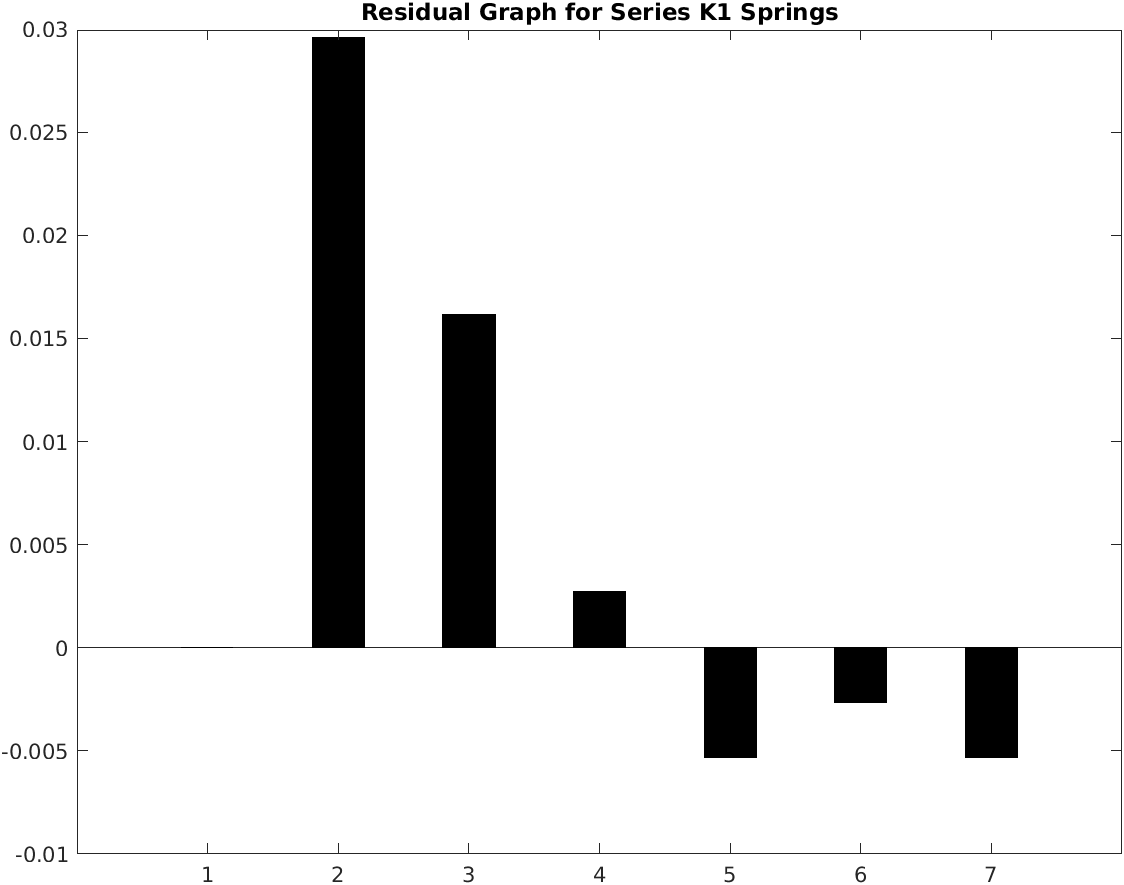
\includegraphics[width=\textwidth]{figures/K1_Se_R.png}
    \caption{Residual Plot for K1 Springs in Series}
    \label{fig:k1_Se_R}
\end{figure}
\end{center}

%%% K2 Single

\begin{center}
\begin{figure}[h!]
    \centering
    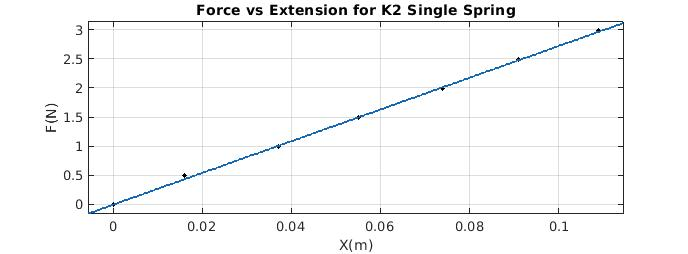
\includegraphics[width=\textwidth]{figures/K2_Single.jpg}
    \caption{Graph of Force vs Extension for Single Spring K2}
    \label{fig:k1_Se_R}
\end{figure}
\end{center}

$$ K2_{single} = 27.25 N/m $$

\newpage
\begin{center}
\begin{figure}[h!]
    \centering
    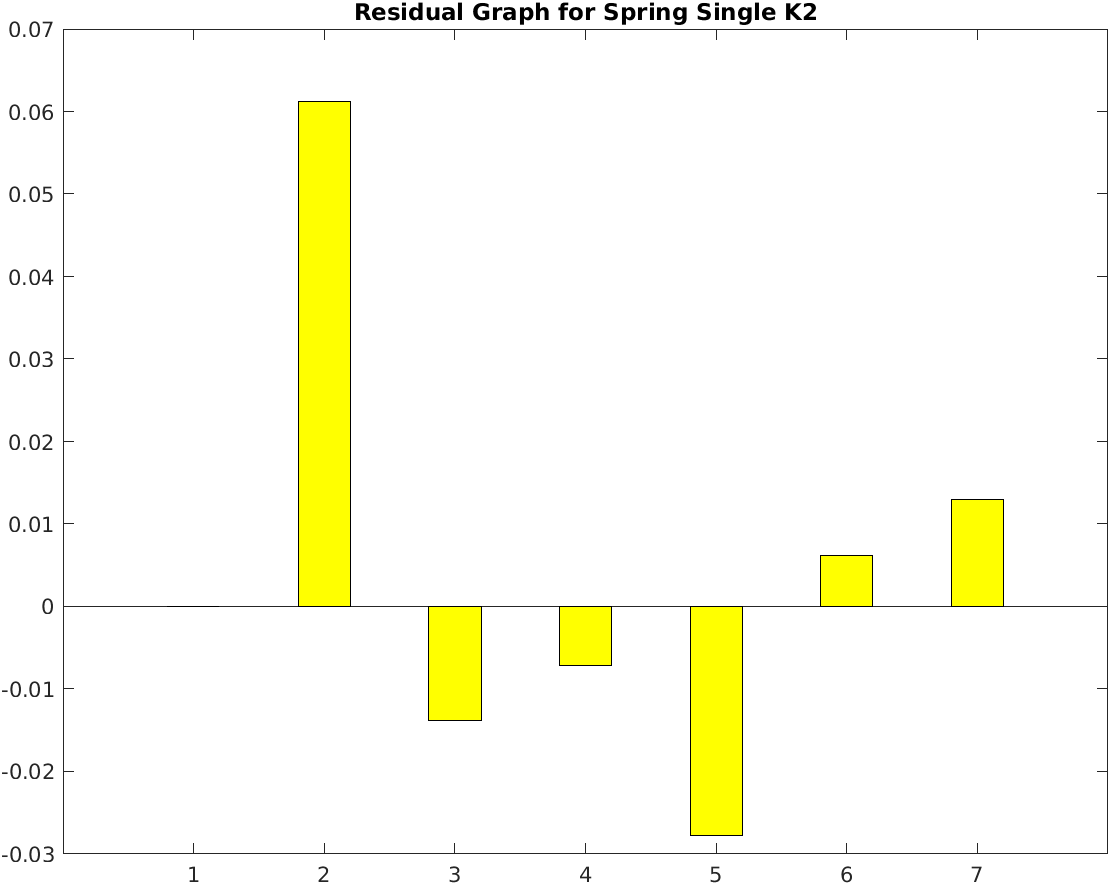
\includegraphics[width=\textwidth]{figures/k2_single.png}
    \caption{Residual Plot for Single K2 Spring}
    \label{fig:k1_Se_R}
\end{figure}
\end{center}

%%%% K2 Series

\begin{center}
\begin{figure}[h!]
    \centering
    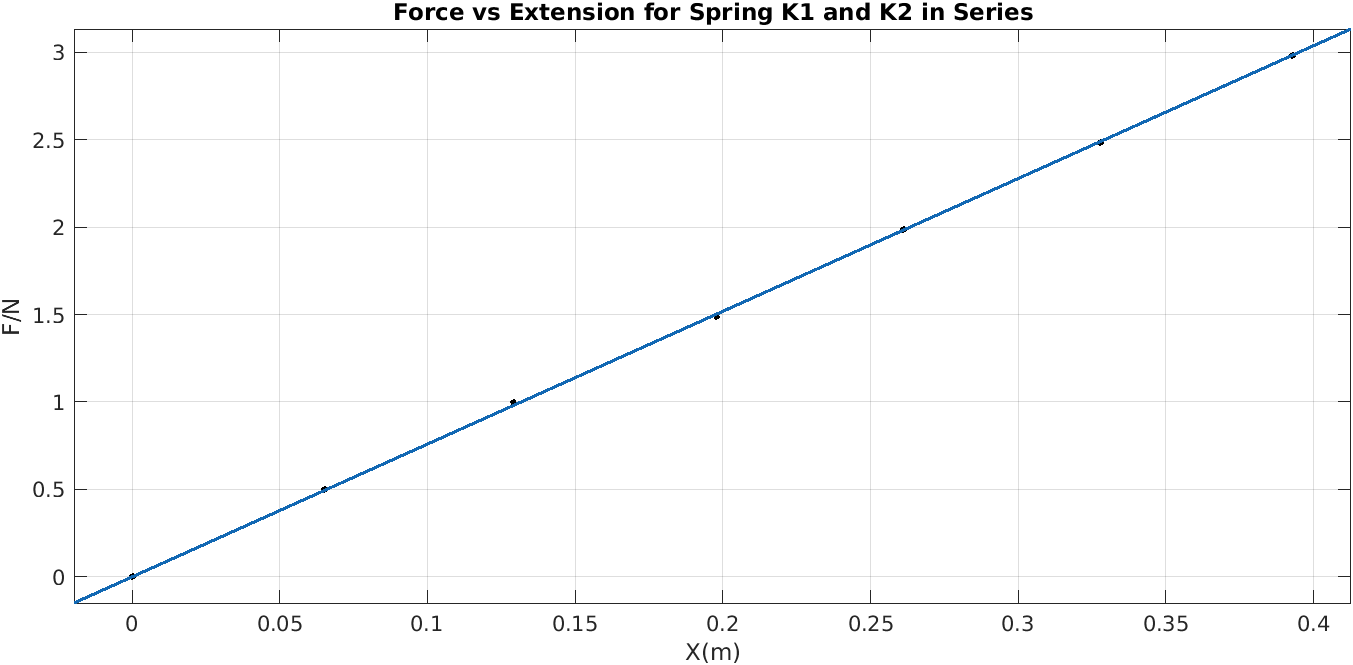
\includegraphics[width=\textwidth]{figures/k1_k2_ser.png}
    \caption{Graph of Force vs Extension for Spring K1 and K2 in series}
    \label{fig:k1_Se_R}
\end{figure}
\end{center}

$$ {K1 and K2}_{series} = 7.593 N/m $$

\begin{center}
\begin{figure}[h!]
    \centering
    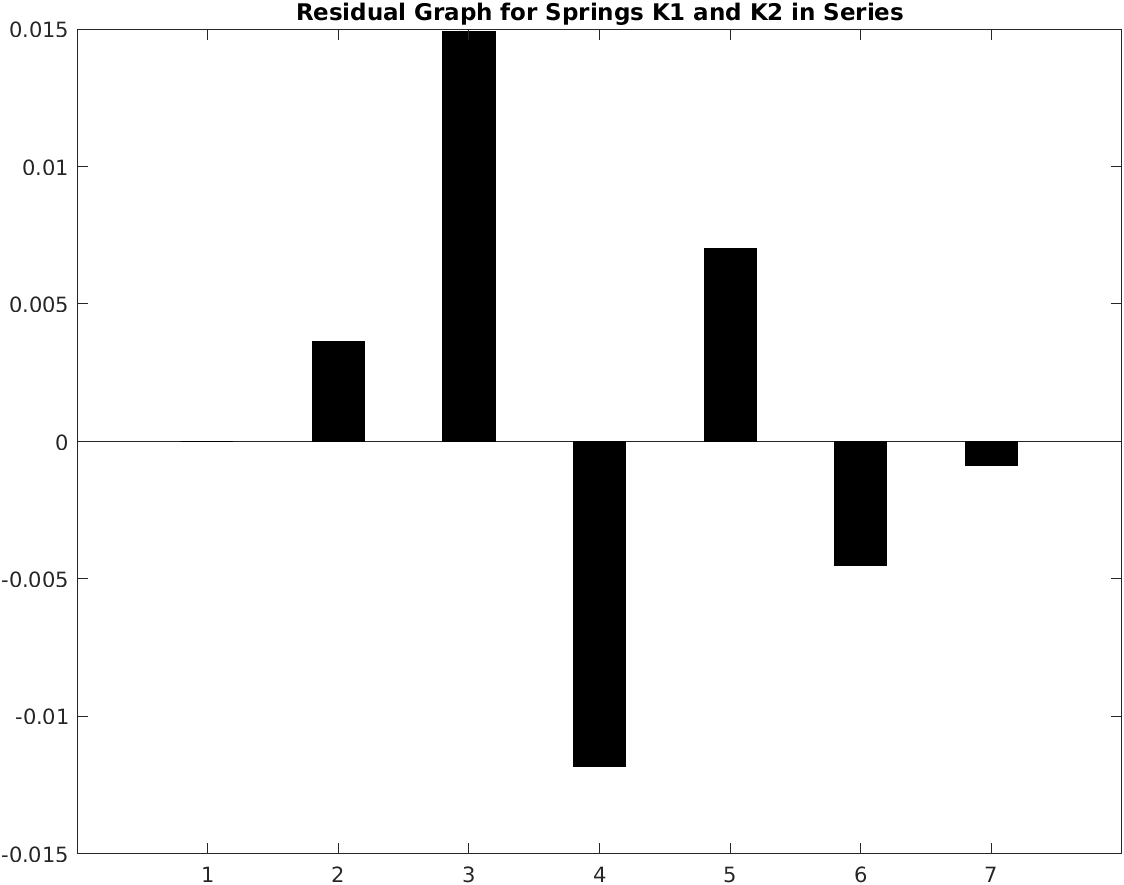
\includegraphics[width=\textwidth]{figures/K1_K2_Series_R.png}
    \caption{Residual Plot for Parallel Springs K1 and K2 in Series}
    \label{fig:k1_Se_R}
\end{figure}
\end{center}

%%%% K2 Parallel
\newpage
\begin{center}
\begin{figure}[h!]
    \centering
    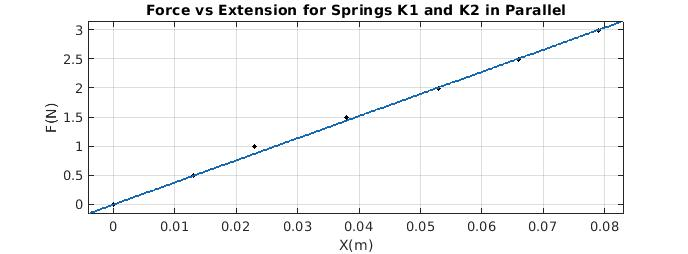
\includegraphics[width=\textwidth]{figures/K1_K2_Parallel.jpg}
    \caption{Graph of Force vs Extension for Springs K1 and K2 in Parallel}
    \label{fig:k1_Se_R}
\end{figure}
\end{center}

$$ {K1 and K2}_{Parallel} = 38.02 N/m $$


\begin{center}
\begin{figure}[h!]
    \centering
    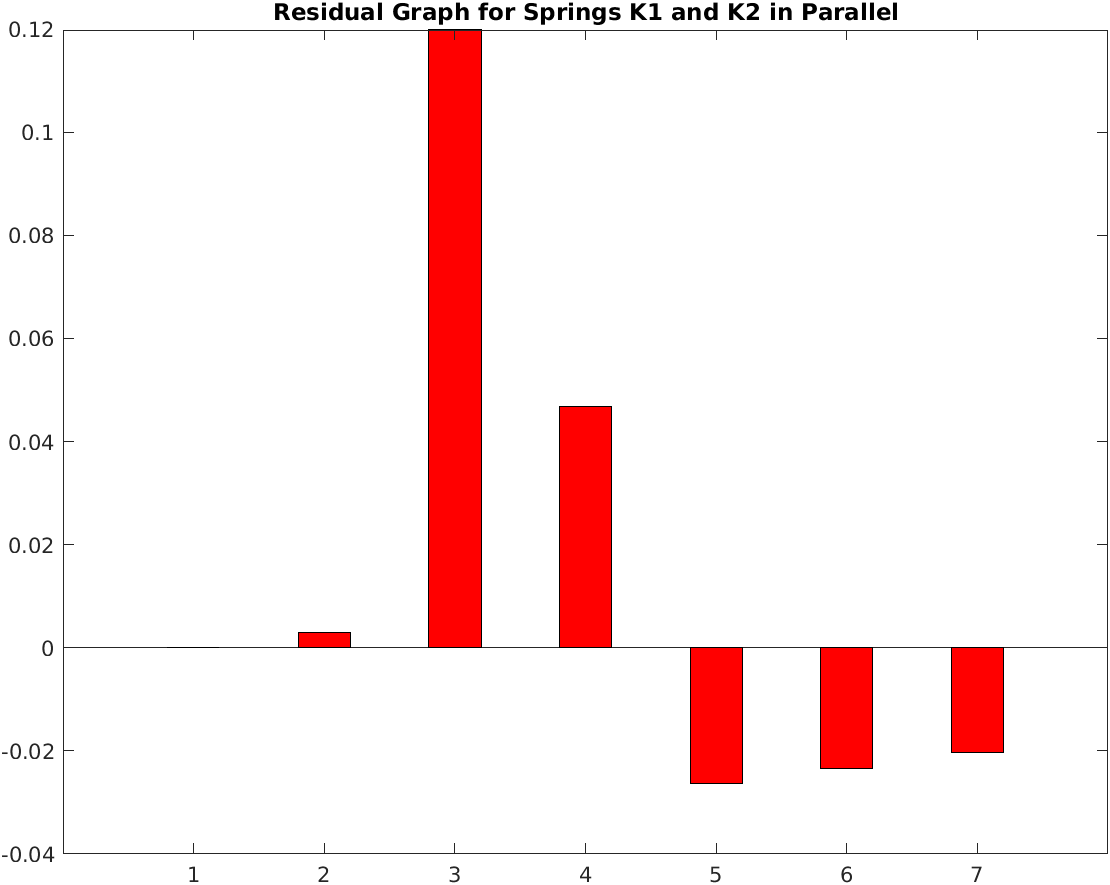
\includegraphics[width=\textwidth]{figures/K1_K2_Parallel_R.png}
    \caption{Residual Plot for Parallel Springs K1 and K2 in Parallel}
    \label{fig:k1_Se_R}
\end{figure}
\end{center}
Theoretical value of K1 and K2 in series = $ 7.695 N/m$ \\
Theoretical value of K1 and K2 in Parallel = $ 37.97 N/m$ \\

\section{Discussion \& Conclusion}
The theoretical and experimental values are the following: 7.593 experimental and 7.695 is experimental values of spring constant for series, they have an error of 0.1 which is quite small. For parallel experimental value is 38.02 and theoretical is 37.97, with error of 0.05. We can also see the random pattern in the residual plots that indicate random errors. Our experimental values are closely matching with theoretical values so our hypothesis is supported by this experiment. \\
 Possible factors of uncertainty and errors can be varying shape of spring, if we attach weights that exceed the springs the springs elastic limit then the spring can deform.
 
 

% Summarize and discuss the experimental results, what do the results say about your hypothesis, if such a hypothesis was made for the experiment. Mention the uncertainty in the calculated quantity Be precise and only include scientific discussion.


\section{MATLAB Script}
\lstinputlisting{matlabCodes/Experiment2.m}





\chapter{Damping constant of a damped harmonic
oscillator}

Date: 21/9/2020

\section{Aim}

In the experiment we aim to measure the damping constant by examining the amplitude of an under damped harmonic oscillator in air using different length pendulums. We observe the change in frequency and model it against curve fitting using data from CASSY software.    



\section{Background Theory}

Acceleration in Simple Harmonic Motion is proportional to the displacement from the start position with a negative sign. When an object that is oscillating moves towards its extreme the negative sign slows it and speeds it up when it is near the mean position. Mathematically, position of pendulum is
$$ x(t)= x_0 \cos(\omega t + \phi)$$ 
with $x_0$ as distance of pendulum from center that is maximum, $\omega$ is a constant and $\phi$ is phase angle. These characteristics are without damping where amplitude remains constant.
For a damped harmonic oscillator, damping force is 
$$F_{damping} = -b v(t)$$ where it is linearly scaled and dependent on speed. Damping constant gives an equation of 
$$m \frac{d^2 x(t)}{dt^2} + b \frac{dx(t)}{dt} + \omega^2 x(t)=0 $$ 
To check whether oscillator is under damped the condition $b^2 - 4m\omega^2$ $<$ 0 should be satisfied and $b^2 - 4m\omega^2$ $>$ 0 and $b^2 - 4m\omega^2$ $=$ 0 holds for over damped and critically damped oscillator. 
Equation of motion for a damped oscillator is 
$$x(t) = A exp(- \gamma t) \cos(\Omega t +\phi)$$ where $\gamma$ is damping constant and  $\Omega$ is frequency of damped oscillator. They are given by the following equations:
$\gamma= b / 2m$ and $\Omega = \sqrt{b^2 -4m\omega^2}$

\section{Description of Setup}
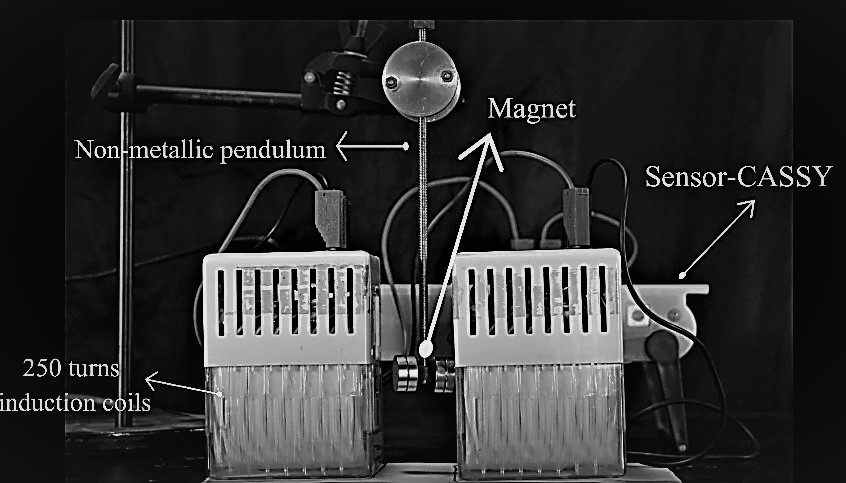
\includegraphics[width=10cm, height=7cm]{figures/fig4.jpeg} \\
 A Non-metallic pendulum is suspended with two magnets, two 250 turns induction coils and a CASSY Sensor is attatched as above to record the motion and amplitude of the oscillator that is damped in air.A rule was used to take the measurement of the length of the pendulum. 


\section{Method / Procedure}

The length of the pendulum is measured using the metre Rule. The two coils were placed close to the magnets and the pendulum was oscillated. CASSY was used to record the data for 50 seconds to view damping. The same process is repeated 3 times for different pendulum lengths. \\
Data of the length of pendulum and its amplitude with time was collected to analyse damping.

\section{Data}

Since the length of the pendulum was only measured once , it does not have type A uncertainty. The type B uncertainty associated is 0.0002m.

\begin{figure}[h!]
    \centering
    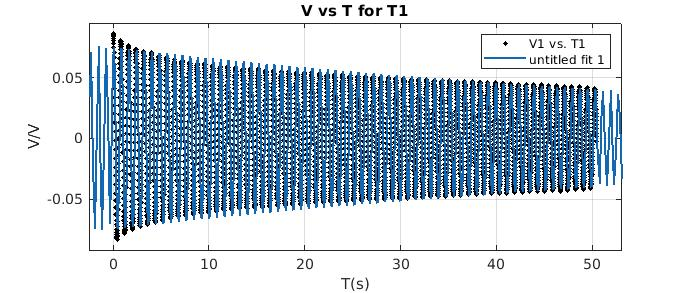
\includegraphics[width=\textwidth]{figures/L1.jpg}
    \caption{Graph of V vs T}
    \label{fig:yx}
\end{figure}
$$ x(t) = 0.07449^{-0.01244t} \times cos(7.873t -0.08103) $$
\newpage
\begin{figure}[h!]
    \centering
    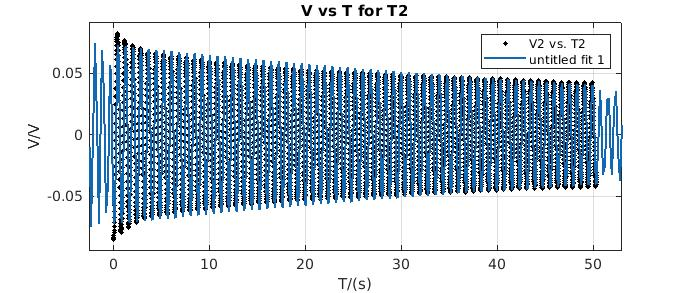
\includegraphics[width=\textwidth]{figures/L2.jpg}
    \caption{Graph of V vs T}
    \label{fig:yx}
\end{figure}
%m_v2 = -0.07236*exp(-0.01184.*T2).*cos(7.882.*T2-0.42);
$$ x(t) = -0.07236^{-0.01184t} \times cos(7.882t -0.42) $$
\newpage
\begin{figure}[h!]
    \centering
    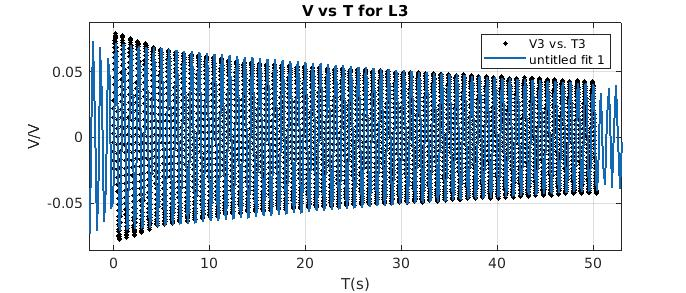
\includegraphics[width=\textwidth]{figures/L3.jpg}
    \caption{Graph of V vs T}
    \label{fig:yx}
\end{figure}
%m_v3 = 0.07135*exp(-0.01141.*T3).*cos(7.965.*T3-1.922);
$$ x(t) = 0.07135^{-0.01141t} \times cos(7.965t - 1.922)$$
\newpage\begin{figure}[h!]
    \centering
    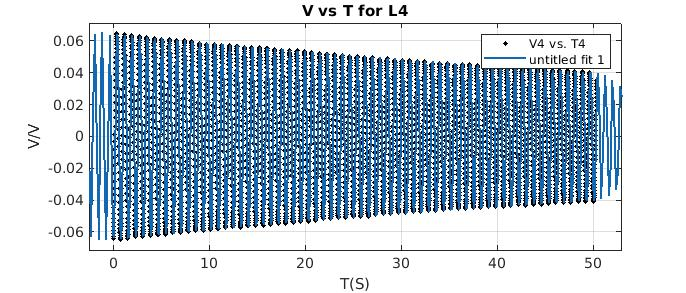
\includegraphics[width=\textwidth]{figures/L4.jpg}
    \caption{Graph of V vs T}
    \label{fig:yx}
\end{figure}
%m_v4 = -0.06439*exp(-0.009528.*T4).*cos(8.031*T4-0.1526);
$$ x(t) = -0.06439^{-0.009528t} \times cos(8.031t - 0.1526)$$
\newpage
\begin{figure}[h!]
    \centering
    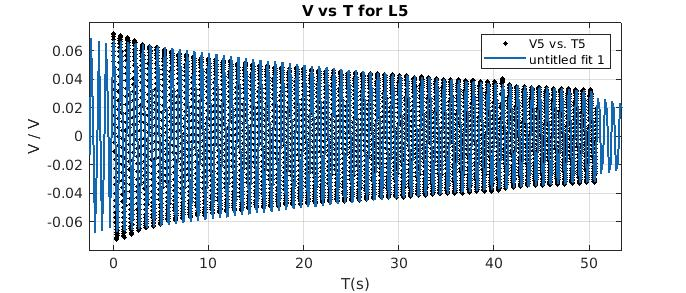
\includegraphics[width=\textwidth]{figures/L5.jpg}
    \caption{Graph of V vs T}
    \label{fig:yx}
\end{figure}
%m_v5 = 0.0673*exp(-0.01495.*T5).*cos(8.142.*T5 - 0.07685);
$$ x(t) = 0.0673^{-0.01495t} \times cos(8.142t - 0.07685)$$
\section{Data Analysis}

\begin{figure}[h!]
    \centering
    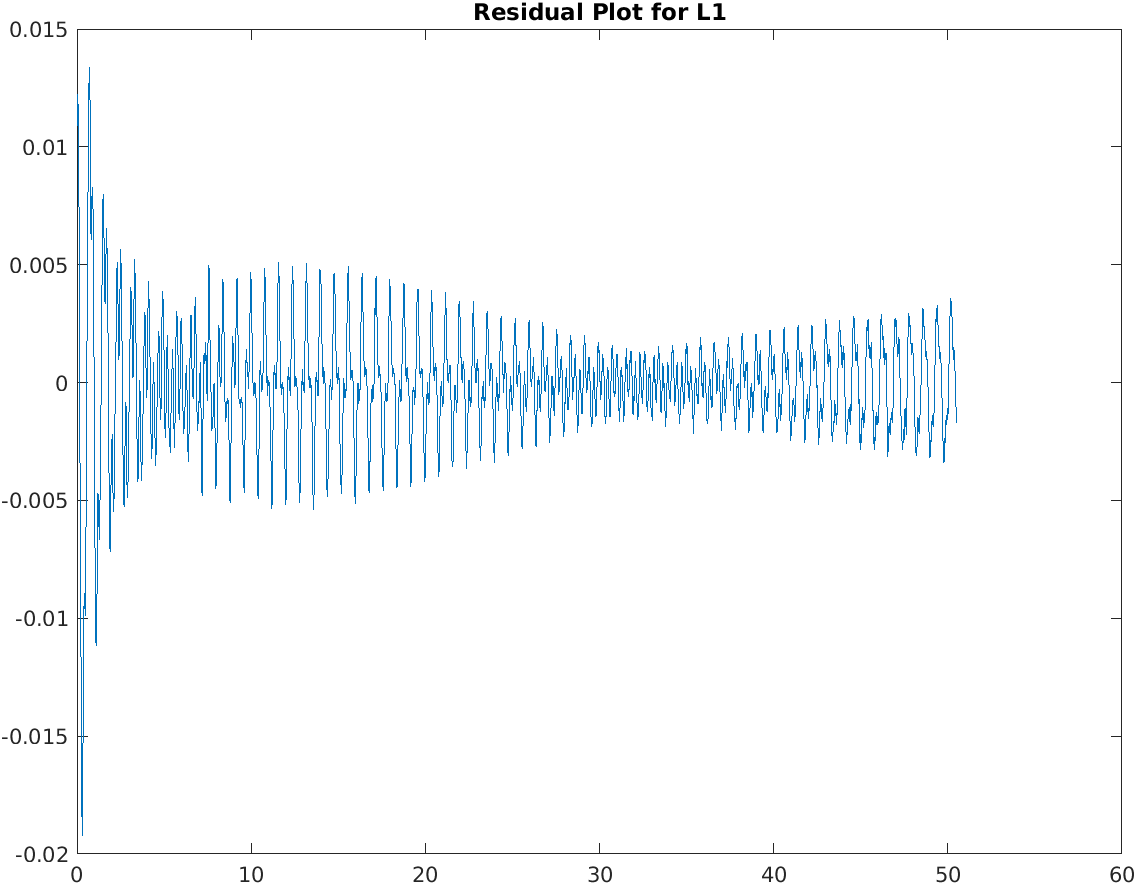
\includegraphics[width=\textwidth]{figures/L1_R.png}
    \caption{Residual Plot for L1}
    \label{fig:yx}
\end{figure}
\newpage
\begin{figure}[h!]
    \centering
    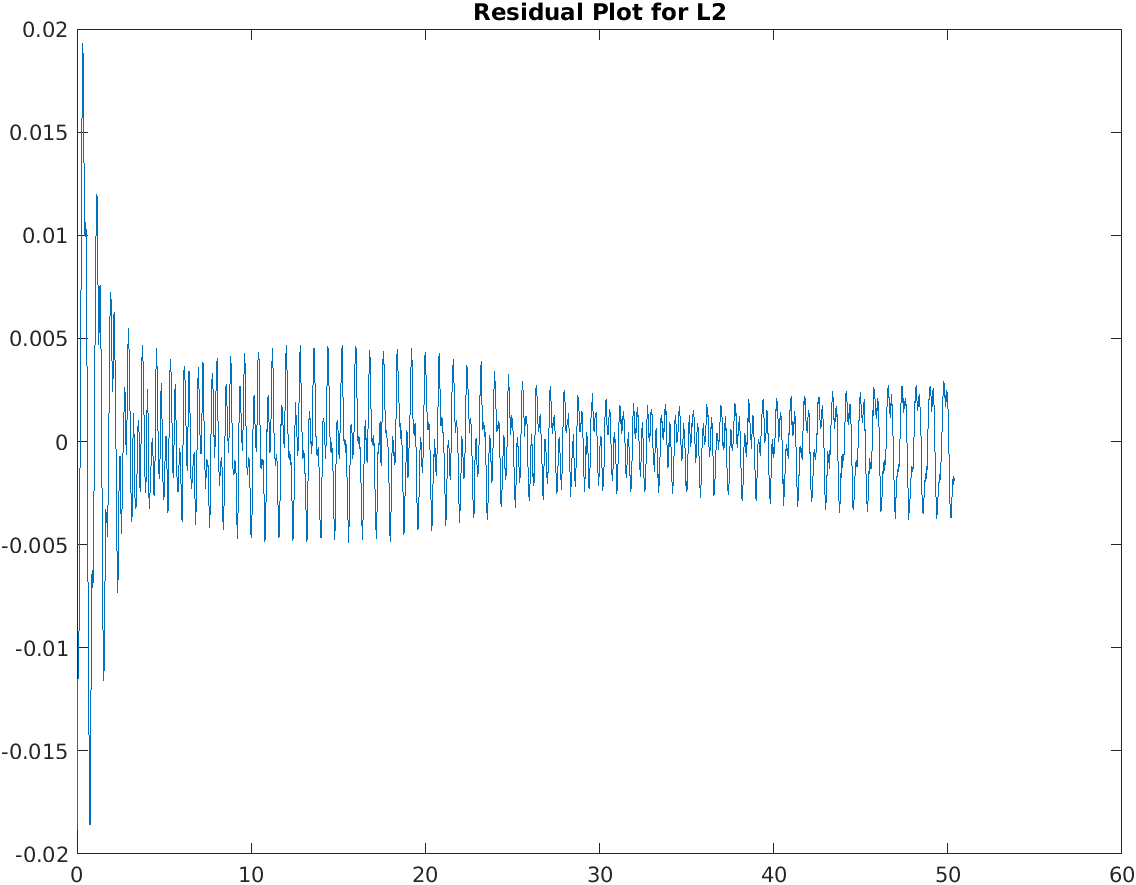
\includegraphics[width=\textwidth]{figures/L2_R.png}
    \caption{Residual Plot for L2}
    \label{fig:yx}
\end{figure}
\newpage
\begin{figure}[h!]
    \centering
    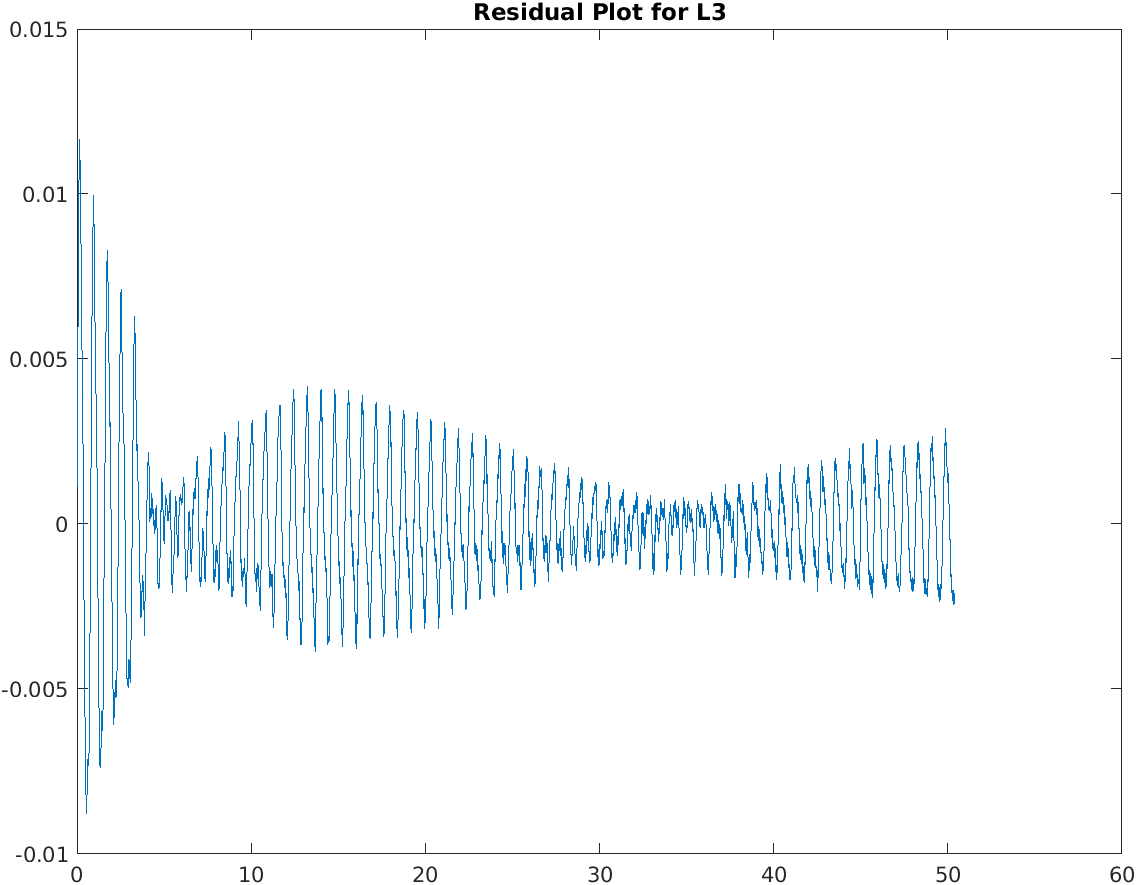
\includegraphics[width=\textwidth]{figures/L3_R.png}
    \caption{Residual Plot for L3}
    \label{fig:yx}
\end{figure}
\newpage
\begin{figure}[h!]
    \centering
    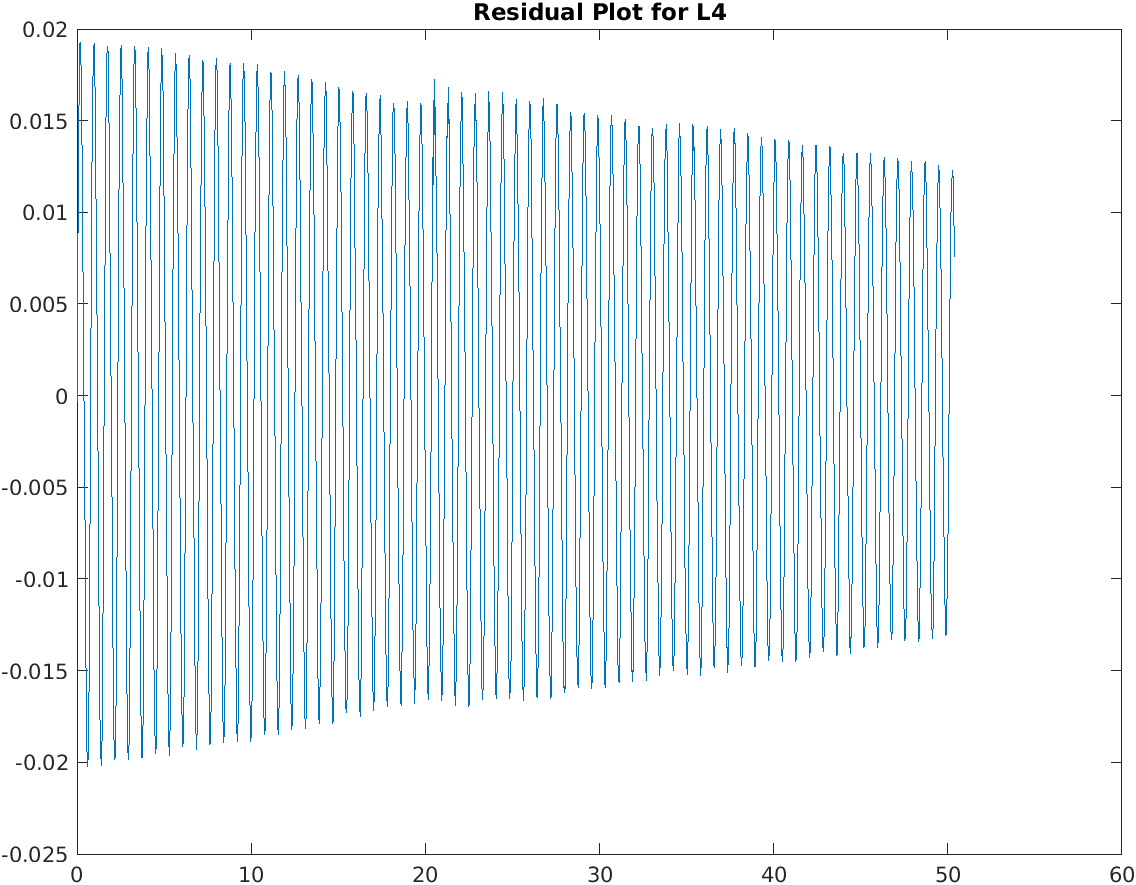
\includegraphics[width=\textwidth]{figures/L4_R.png}
    \caption{Residual Plot for L4}
    \label{fig:yx}
\end{figure}
\newpage
\begin{figure}[h!]
    \centering
    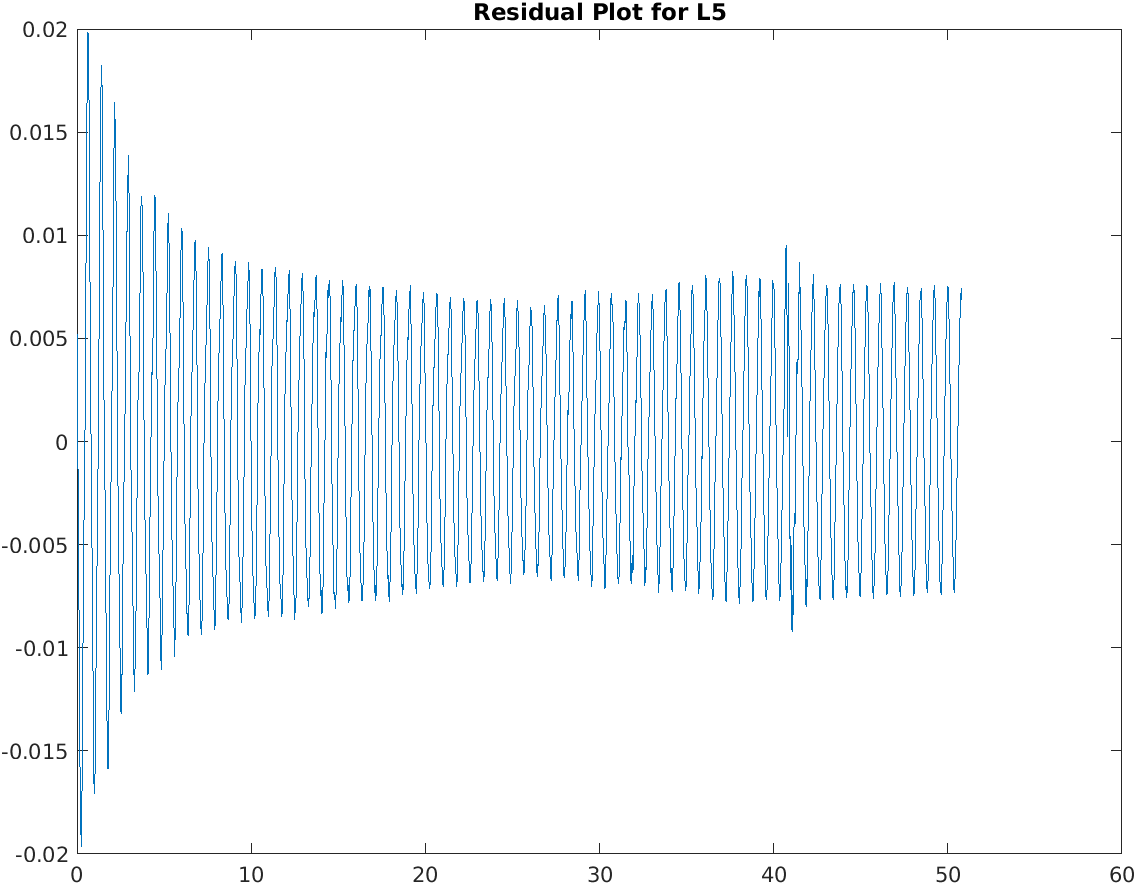
\includegraphics[width=\textwidth]{figures/L5_R.png}
    \caption{Residual Plot for L5}
    \label{fig:yx}
\end{figure}


\newpage
\begin{figure}[h!]
    \centering
    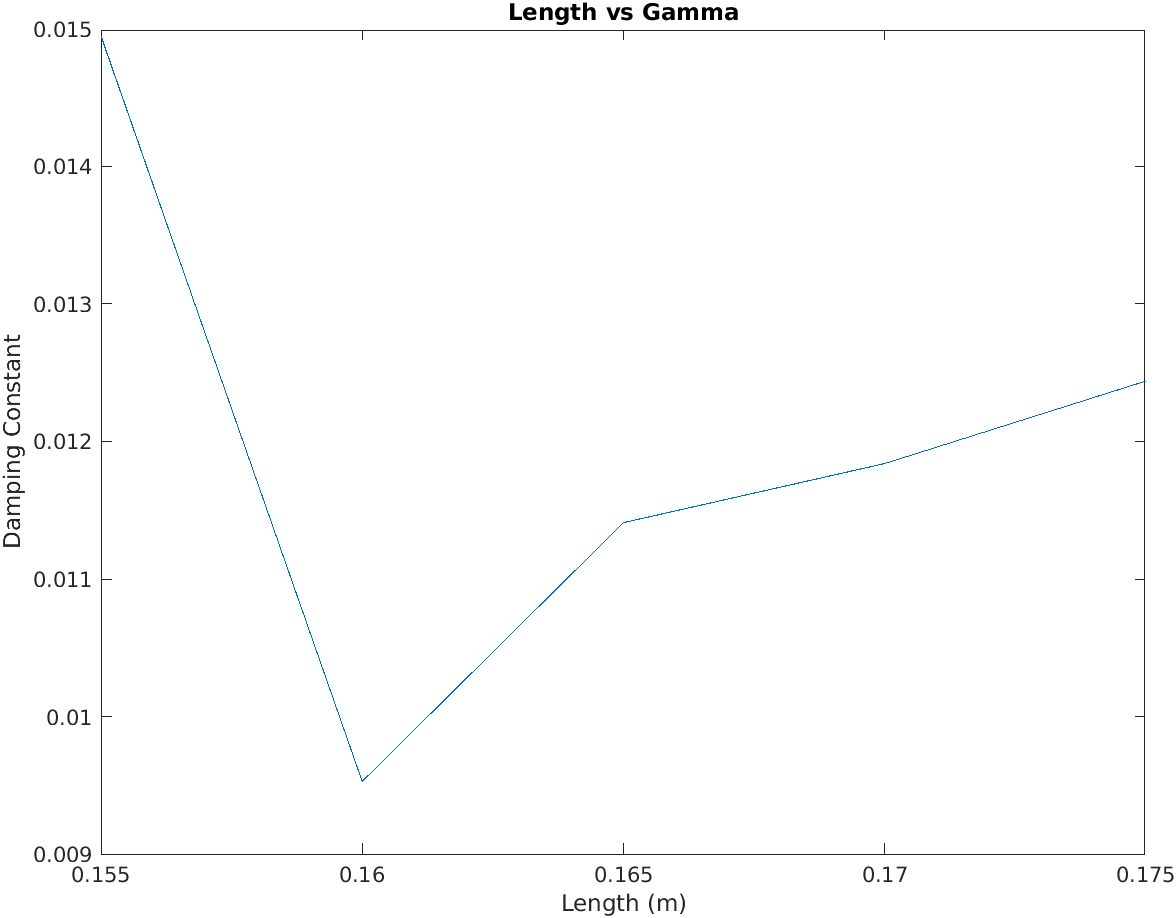
\includegraphics[width=\textwidth]{figures/L vs G.png}
    \caption{Graph of Length  vs Damping Constant}
    \label{fig:yx}
\end{figure}

\section{Discussion \& Conclusion}

The graph of the the damping constants vs length and the residual plots show have random pattern which indicate the presence of random errors. The experiment could have been improved by ensuring that there was no wind in the room while doing the experiment. 


\section{MATLAB Script}
\lstinputlisting{matlabCodes/Experiment3.m}





Date: 15/08/2020

=-\chapter{Energy conservation between 2D motions}

% Date: 5/9/2020

\section{Aim}

In this experiment, our aim is to understand how energy is transferred when objects collide by varying the angle at which an object is released to collide with another.


\section{Background Theory}

 According to principle of physics energy is always conserved in a close system. Therefore, energy can be in different firms but the total energy remains the same. 
Energy for a moving object is kinetic energy and can be calculated using 
$$ E=\frac{1}{2} m v^2$$
and gravitational potential energy is when an object is stationary at a height and is has the ability to move. It is given by the equation $$E=mgh$$
For an object in projectile motion the position of body in x and y position are as following:
$$x(t) =x_0 +v_{0,x}t $$ 
$$y(t)= y_0 +v_{0,y}t -\frac {1}{2}gt^2$$
There is no acceleration in the horizontal direction, just a constant velocity but in the vertical direction there is constant acceleration. 
When two objects collide, the distance that the ball will reach the ground is 
$$d=2\sqrt{hL(1-\cos(\theta)}$$ where h denotes height pf collision, L is length of pendulum, $\theta$ is angle from which the swinging pendulum is placed. 

\section{Description of Setup}
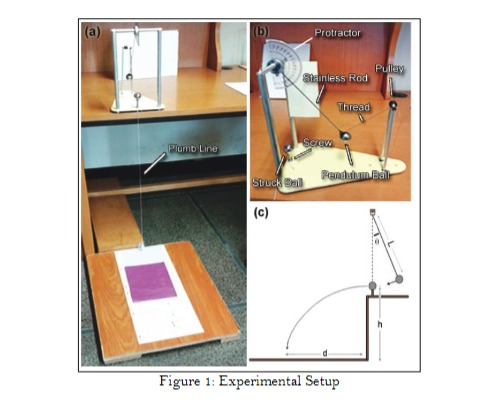
\includegraphics[width=10cm, height=7cm]{figures/figm.jpeg} \\
Here a pendulum is strung over a pulley with a fixed protractor and a metal ball is placed as shown in the figure. White sheets are placed below with a carbon paper on top to locate the position of the ball when released. A meter rule is also required.

\section{Method / Procedure}
The vertical height from the center of the ball to the ground is measured and marked. White papers are fixed to the ground with carbon paper on top. 
The pendulum is held at a high position at an angle of 30 measured through the fixed protractor on the pendulum and swung. It strikes the ball which follows a parabolic path and strikes the carbon sheet placed on the white papers on the floor. Repeat this process four times at the same angle. 
The same steps should be repeated at an angle of 40, 50 and 60 degrees and 5 readings should be taken at each angle. The length, d, of all the points of impact from initial position is measured and compared with theoretical predictions.  . 


\section{Data}

In this experiment, the constants h and L were only measured once and therefore don't have any Type A uncertainty. The type B uncertainty associated with both h and L is respectively  0.0002m. Consequently, $ h = 0.935 \pm 0.0002$m and $ L = 0.25 \pm 0.0002m $. The angle $\theta$ was also only measured only it doesn't have type A uncertainty. The type B associated with the angle $\theta $ is $ 0.04 $ degrees. The distance d was measured multiple and therefore it has both type B and type A uncertainty.
The recorded values for the angle $\theta$
\begin{center}
\begin{tabular}{|c|c|c|}
\hline
\textbf{s.No} & \textbf{Angle} & \textbf{angle (°)} \\ \hline
1             & A1             & 30                 \\ \hline
2             & A2             & 40                 \\ \hline
3             & A3             & 50                 \\ \hline
4             & A4             & 60                 \\ \hline
\end{tabular}
\end{center}

The values measured for the distance d (cm).
\begin{center}
\begin{tabular}{|l|l|l|l|l|}
\hline
\textbf{s.No} & \textbf{d\_A1 (cm)} & \textbf{d\_A2 (cm)} & \textbf{d\_A3 (cm)} & \textbf{d\_A4 (cm)} \\ \hline
1             & 30.5                & 42.7                & 55                  & 64.7                \\ \hline
2             & 31.5                & 43.3                & 55.7                & 63.8                \\ \hline
3             & 31.8                & 43                  & 57.7                & 65.4                \\ \hline
4             & 32.7                & 44.6                & 54                  & 65.3                \\ \hline
5             & 31.4                & 43.5                & 54.8                & 64.7                \\ \hline
\end{tabular}
\end{center}
Type A uncertainty in distance d when Angle($\theta = 30$)
\begin{center}
$\sigma_d = 0.0071m$ \\
$ U_d^A =  0.0035m$ \\
\end{center}
Type A uncertainty in distance d when Angle($\theta = 40$)
\begin{center}
$\sigma_d = 0.0065m$ \\
$ U_d^A =  0.0032m$ \\
\end{center}
Type A uncertainty in distance d when Angle($\theta = 50$)
\begin{center}
$\sigma_d = 0.0125m$ \\
$ U_d^A =  0.0063m$ \\
\end{center}
Type A uncertainty in distance d when Angle($\theta = 60$)
\begin{center}
$\sigma_d = 0.0057m$ \\
$ U_d^A =  0.0029m$ \\
\end{center}



\section{Data Analysis}
We will calculate the expected value for d using the following formula
    $$ d = 2 \sqrt{hL(1-cos(\theta))}$$
where h and L are constants with the values $ h = 0.935m$ and $L = 0.25m$\\

\begin{center}
\begin{tabular}{|l|l|l|}
\hline
s.No & Angle(°) & Expected value of d(m) \\ \hline
1    & 30       & 0.3539                 \\ \hline
2    & 40       & 0.4677                 \\ \hline
3    & 50       & 0.5779                 \\ \hline
4    & 60       & 0.6837                 \\ \hline
\end{tabular}
\end{center}

Average Value of the distance d for each value of the Angle($\theta$)
\begin{center}
\begin{tabular}{|l|l|l|l|}
\hline
s.No & Angle(°) & Avg\_d (cm) & Avg\_d(m) \\ \hline
1    & 30       & 31.58       & 0.316     \\ \hline
2    & 40       & 43.42       & 0.434     \\ \hline
3    & 50       & 55.44       & 0.554     \\ \hline
4    & 60       & 64.78       & 0.648     \\ \hline
\end{tabular}
\end{center}

\newpage
The graph of average distance d  vs Angle ($\theta$)
\begin{figure}[h!]
    \centering
    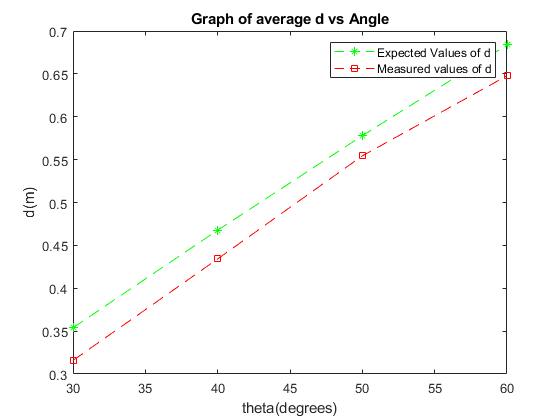
\includegraphics[width=\textwidth]{figures/Avg_d_vs_theta.png}
    \caption{Graph of Average d vs Angle ($\theta$)}
    \label{fig:yx}
\end{figure}
\newpage
Residual plot for d as when $\theta = 30 $
\begin{figure}[h!]
    \centering
    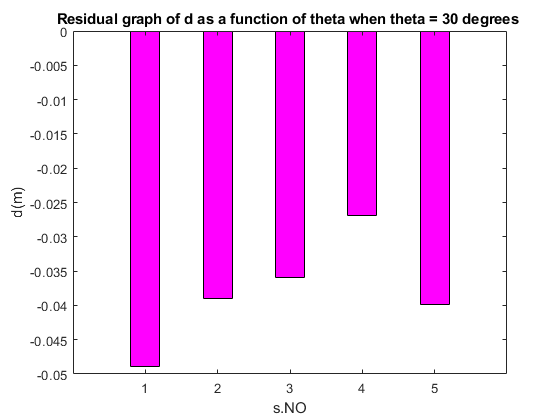
\includegraphics[width=\textwidth]{figures/d_A1_r.png}
    \caption{Residual Plot for  d when Angle ($\theta$ = 30)}
    \label{fig:yx}
\end{figure}
\newpage
Residual plot for d as when $\theta = 40 $
\begin{figure}[h!]
    \centering
    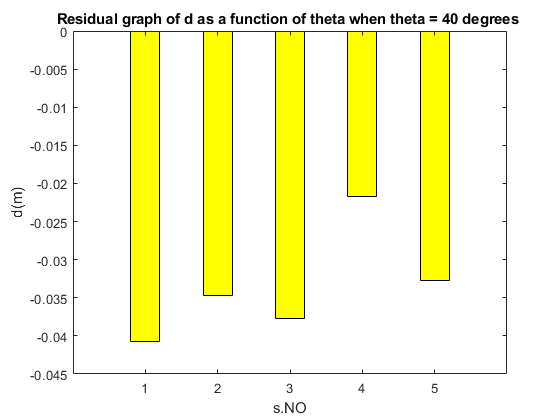
\includegraphics[width=\textwidth]{figures/d_A2_r.png}
    \caption{   Residual Plot for d when Angle($\theta$ = 40)}
    \label{fig:yx}
\end{figure}
\newpage 
Residual plot for d as when $\theta = 50 $
\begin{figure}[h!]
    \centering
    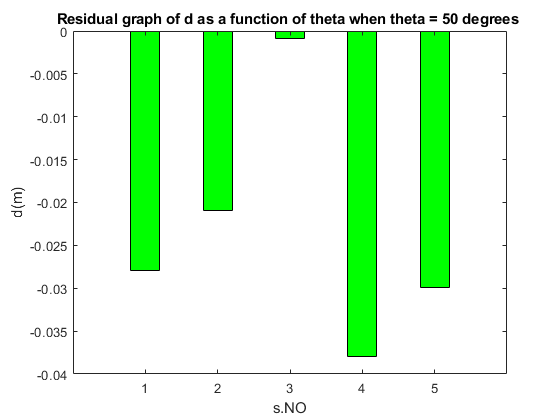
\includegraphics[width=\textwidth]{figures/d_A3_r.png}
    \caption{Residual Plot for  d when Angle ($\theta$ = 50)}
    \label{fig:yx}
\end{figure}
\newpage 
Residual plot for d as when $\theta = 60 $
\begin{figure}[h!]
    \centering
    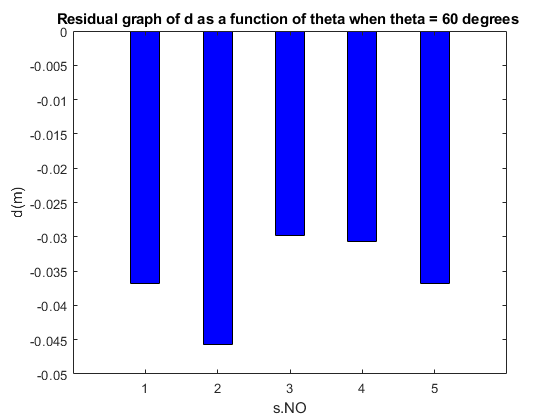
\includegraphics[width=\textwidth]{figures/d_A4_r.png}
    \caption{Residual Plot for d when Angle  ($\theta = 60$) }
    \label{fig:yx}
\end{figure}
We can transfer uncertainty from Angle($\theta$) to distance (d) using the following formula:
$$ U_d = \sqrt{{U_T^A}^2 +{U_T^B}^2+\biggr({\frac{\sqrt{hL}sin(\theta)\Delta\theta}{\sqrt{1-cos(\theta)}}}\biggr)^2}$$

\begin{center}
\begin{tabular}{|l|l|l|}
\hline
Expected value of   d(m) & Total Uncertainty in d(m) & Final Value(m)                     \\ \hline
0.316                    & 0.0272                     & $0.316 \pm 0.027$ \\ \hline
0.434                    & 0.0264                     & $ 0.434\pm 0.026$   \\ \hline
0.554                    & 0.0261                     & $ 0.554\pm 0.061$   \\ \hline
0.648                    & 0.0243                     & $ 0.648\pm 0.024$   \\ \hline
\end{tabular}
\end{center}
\newpage
\begin{figure}[h!]
    \centering
    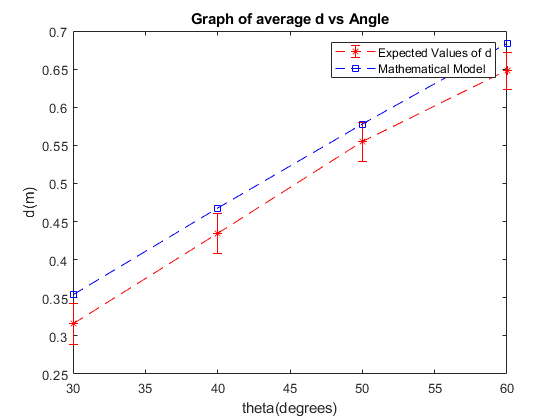
\includegraphics[width=\textwidth]{figures/Mathematical_Model.png}
    \caption{Graph of d vs Angle($\theta$)}
    \label{fig:yx}
\end{figure}


\section{Discussion \& Conclusion}
For our experiment and data, we can evaluate that at angle 30, theoretical value of d should be 0.3539 and our experimental value is 0.316 with error of 0.027. The theoretical value does not lie in the range $0.316 \pm 0.027$. Whereas for angle of 40, and 50 it does but not 60. We can also see that all our measured values are below expected values of d from figure 4.1. This implies that it is difficult to conclude if hypothesis is valid because half values agree with theoretical values. Possible factors of uncertainty could be wind and parallax errors in measuring the distances using metre rule. Air resistance could also cause experimental values to be less than the theoretical values since it acts as an opposing force. Furthermore, it may be difficult to locate exact location of where the ball may have struck first as it may touch several points on the carbon paper. A more accurate set up could have given results with the hypothesis that could include wind blockers, a camera or motion detector to ensure exact location of contact can be recorded. To deduce a better conclusion, the experiment should be carried out on multiple angles or in a setup to minimize air resistance so that a conclusion may be reached.     

% Summarize and discuss the experimental results, what do the results say about your hypothesis, if such a hypothesis was made for the experiment. Mention the uncertainty in the calculated quantity Be precise and only include scientific discussion.


\section{MATLAB Script}
\lstinputlisting{matlabCodes/Experiment4.m}


%\clearpage
%\thispagestyle{empty}
%\null

\chapter{Conservation of Linear Momentum}

Date: 29/10/2020

\section{Aim}

In this experiment we aim to observe the final velocities of two trolleys, on a track using light gates, that are colliding elastically and in-elastically by varying their masses. We observe their initial velocity and make inferences using data from CASSY software. 


\section{Background Theory}

We define Linear momentum for a object of mass m kg and velocity $\vec{v}$ to be 
$$ \vec{p} = m \times \vec{v} $$
The principle of conservation of momentum states that ``If no net force acts upon a system, then there is no change in the total momentum of the system.''. This can be expressed mathematically as 
$$ \vec{p_{initial}} = \vec{p_{final}}$$
In case of an elastic collision, the total momentum and the kinetic energy before and after the collision is conserved. This can be expressed as 
$$ m_1 \times \vec{v_{i^1}} +  m_2 \times \vec{v_{i^2}} =  m_1 \times \vec{v_{f^1}} +  m_2 \times \vec{v_{i^2}}$$
$$ \frac{1}{2} \times( m_1 \times (\vec{v_{i^1}})^2 +  m_2 \times (\vec{v_{i^2}})^2 ) =  \frac{1}{2} \times( m_1 \times (\vec{v_{f^1}})^2 +  m_2 \times (\vec{v_{i^2}})^2) $$
In case of an in-elastic collision, only the total momentum is conserved. This can be expressed as 
$$ m_1 \times \vec{v_{i^1}} +  m_2 \times \vec{v_{i^2}} =  (m_1 + m_2 ) \times\vec{v_f}$$

Elastic Collision and $m1 = m2$ . 
\begin{center}
    \begin{itemize}
        \item $ \vec{v_{f^1}} = \vec{v_{i^2}}$
        \item $ \vec{v_{f^2}} = \vec{v_{i^i}}$
    \end{itemize}
\end{center}

Elastic Collision and $m1 \neq m2$ . 
\begin{center}
    \begin{itemize}
        \item $ \vec{v_{f^1}} = \frac{m_1 - m_2}{m_1+m_2} \times \vec{v_{i^i}} +  \frac{2 \times m_2 \vec{v_{i^2}}}{m1+m2}$
        \item $ \vec{v_{f^2}} = \frac{m_2 - m_1}{m_1+m_2} \times \vec{v_{i^1}} +  \frac{2 \times m_1 \vec{v_{i^1}}}{m1+m2}$
    \end{itemize}
\end{center}
In-Elastic Collision and $m1 = m2$ . 
\begin{center}
    \begin{itemize}
        \item $ \vec{v_{f}} = 0.5 \times \vec{v_{i^2}}$
    \end{itemize}
\end{center}
In-Elastic Collision and $m1 \neq m2$ . 
\begin{center}
    \begin{itemize}
        \item $ \vec{v_{f}} = \frac{(m_1 \times \vec{v_{i^1}} +  m_2 \times \vec{v_{i^2}})}{m_1 + m_2}$
    \end{itemize}
\end{center}

\section{Description of Setup}
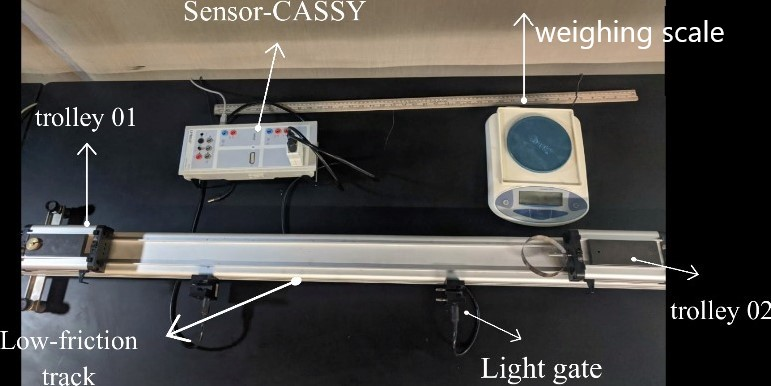
\includegraphics[width=15cm, height=8cm]{figures/exp5fig.jpeg} \\
In the setup above two trolleys with additional weights are placed on a track with light gates. Cassy Software is attached to record data and an electronic balance is used to measure the mass of trolleys.  

% Sketch and explain the experimental setup. The explanation should try to cover these pointers:  table \ref{tab:addlabel}
% \begin{enumerate}
%     \item What is the purpose of individual items in the setup?
%     \item If any equipment is taking measurements, what is it reading and how is it being read?
% \end{enumerate}

% Be precise to, ONLY include scientific description.

\section{Method / Procedure}
The CASSY software settings were set up for the conservation of momentum. The masses of trolleys were measured using the balance alongside the spring for elastic collision and the two trolleys were pushed to collide elastically with equal masses. This was repeated five times. Elastic collision was also performed using unbalanced masses and velocities data was seen through CASSY. The same procedure was repeated for inelastic collision with equal masses and unequal masses five times respectively. CASSY was used to collect the data of masses of trolleys and initial and final velocities of trolleys before and after collisions with the help of light gates. 

% Highlight the following aspects of the experiment conducted 
% \begin{enumerate}
%     \item What method did you use to perform the experiment?
%     \item What adjustments were made, if any? 
%     \item What data was collected?
%     \item How was it collected?
%     \item Were any calibrations made and what were they?
% \end{enumerate}



\section{Data}

\begin{center}
    
\begin{adjustbox}{width=1\textwidth}
\begin{tabular}{|l|l|l|l|l|l|l|}
\hline

\multicolumn{7}{|c|}{\textbf{Elastic Collision (Case a: m1 = m2)}} \\ \hline
Serial No & V1-initial - m/s & V2-initial - m/s & V1-final (experiment) - m/s & V1-final (theoretical) - m/s & V2-final (experiment) - m/s & V2-final (theoretical) - m/s \\ \hline
1   & 0.687   & -0.511   & -0.453   & -0.511   & 0.679   & 0.687   \\ \hline
2   & 0.762   & -0.83    & -0.762   & -0.83    & 0.704   & 0.762   \\ \hline
3   & 0.55    & -0.572   & -0.523   & -0.572   & 0.553   & 0.55    \\ \hline
4   & 0.637   & -0.702   & -0.634   & -0.702   & 0.63    & 0.637   \\ \hline
5   & 0.547   & -0.611   & -0.558   & -0.611   & 0.543   & 0.547   \\ \hline
\end{tabular}
\end{adjustbox}
\end{center}

\begin{center}
\begin{adjustbox}{width=1\textwidth}
\begin{tabular}{|l|l|l|l|l|l|l|}
\hline
\multicolumn{7}{|c|}{\textbf{Elastic Collision (Case b: m1 != m2)}} \\ \hline
Serial No & V1-initial - m/s & V2-initial - m/s & V1-final (experiment) - m/s & V1-final (theoretical) - m/s & V2-final (experiment) - m/s & V2-final (theoretical) - m/s \\ \hline
1  & 0.573  & -0.616  & -0.178 & -0.210155718 & 0.936 & 0.978844282 \\ \hline
2  & 0.594  & -0.538  & -0.154 & -0.151611667 & 0.848 & 0.980388333 \\ \hline
3  & 0.411  & -0.477  & -0.156 & -0.173896785 & 0.691 & 0.714103215 \\ \hline
4  & 0.393  & -0.694  & -0.299 & -0.322971627 & 0.731 & 0.764028373 \\ \hline
5  & 0.491  & -0.566  & -0.18  & -0.205211601 & 0.827 & 0.851788399 \\ \hline
\end{tabular}
\end{adjustbox}
\end{center}

\begin{center}
\begin{adjustbox}{width=1\textwidth}
\begin{tabular}{|l|l|l|l|l|l|l|}
\hline
\multicolumn{7}{|c|}{\textbf{In-Elastic Collision (Case a: m1 = m2)}} \\ \hline
Serial No & V1-initial - m/s & V2-initial - m/s & V1-final (experiment) - m/s & V1-final (theoretical) - m/s & V2-final (experiment) - m/s & V2-final (theoretical) - m/s \\ \hline
1     & 0.535    & 0    & 0.26     & 0.2675    & 0.262    & 0.2675    \\ \hline
2     & 0.677    & 0    & 0.331    & 0.3385    & 0.332    & 0.3385    \\ \hline
3     & 0.693    & 0    & 0.337    & 0.3465    & 0.345    & 0.3465    \\ \hline
4     & 0.584    & 0    & 0.258    & 0.292     & 0.263    & 0.292     \\ \hline
5     & 0.616    & 0    & 0.298    & 0.308     & 0.301    & 0.308     \\ \hline
\end{tabular}
\end{adjustbox}
\end{center}

\begin{center}
\begin{adjustbox}{width=1\textwidth}
\begin{tabular}{|l|l|l|l|l|l|l|}
\hline
\multicolumn{7}{|c|}{\textbf{In-Elastic Collision (Case b: m1 != m2)}} \\ \hline
Serial No & V1-initial - m/s & V2-initial - m/s & V1-final (experiment) - m/s & V1-final (theoretical) - m/s & V2-final (experiment) - m/s & V2-final (theoretical) - m/s \\ \hline
1   & 0.559  & -0.521  & 0.196  & 0.199193133  & 0.196  & 0.199193133  \\ \hline
2   & 0.441  & -0.424  & 0.151  & 0.152821352  & 0.152  & 0.152821352  \\ \hline
3   & 0.512  & -0.511  & 0.172  & 0.17118294   & 0.173  & 0.17118294   \\ \hline
4   & 0.454  & -0.539  & 0.117  & 0.123177575  & 0.12   & 0.123177575  \\ \hline
5   & 0.51   & -0.328  & 0.23   & 0.230816524  & 0.232  & 0.230816524  \\ \hline
\end{tabular}
\end{adjustbox}
\end{center}



\section{Data Analysis}
\newpage
\begin{figure}[h!]
    \centering
    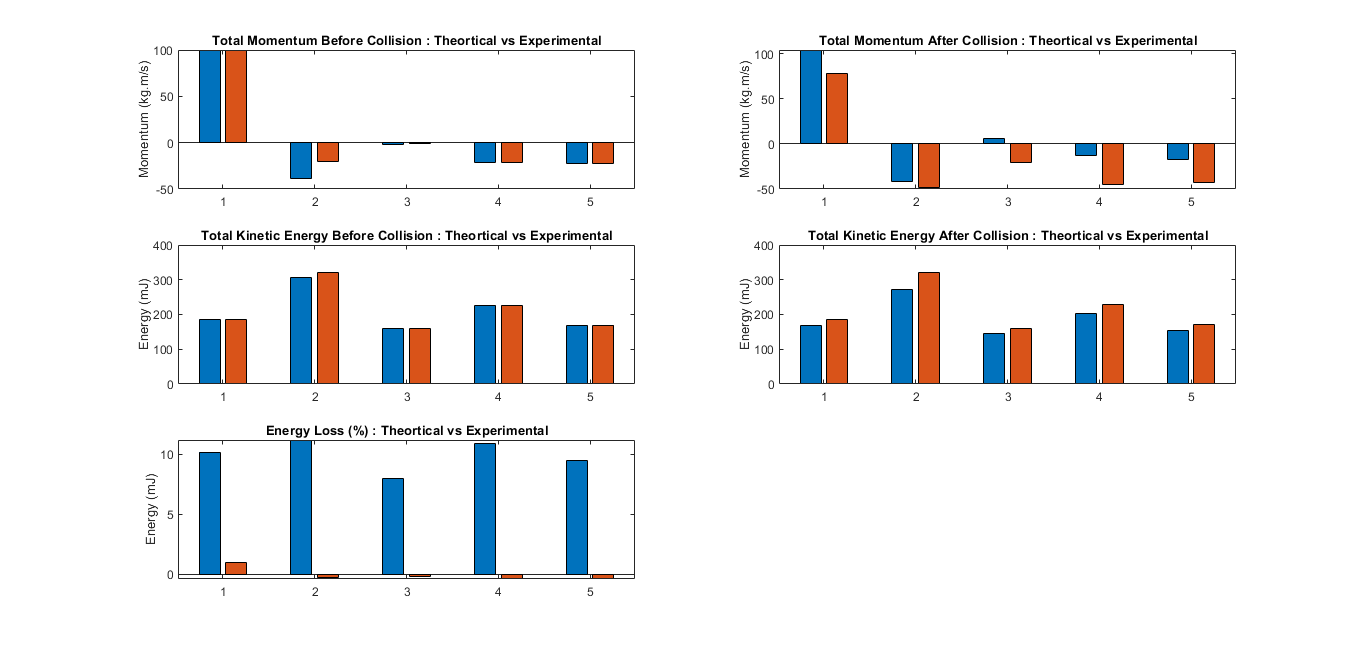
\includegraphics[width=\textwidth]{figures/Exp1.png}
    \caption{Elastic Collision with $m_1 = m_2$}
    \label{fig:yx}
\end{figure}

\newpage
\begin{figure}[h!]
    \centering
    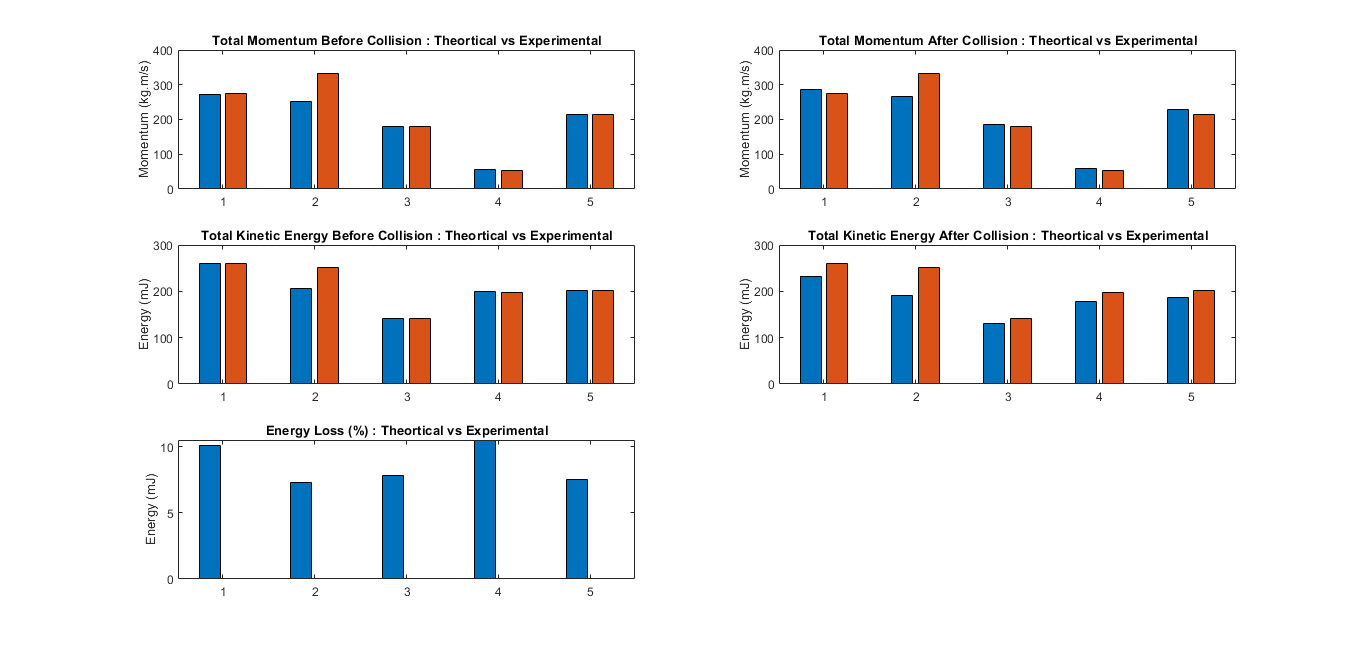
\includegraphics[width=\textwidth]{figures/Exp2.png}
    \caption{Elastic Collision with $m_1 \neq m_2$}
    \label{fig:yx}
\end{figure}

\newpage
\begin{figure}[h!]
    \centering
    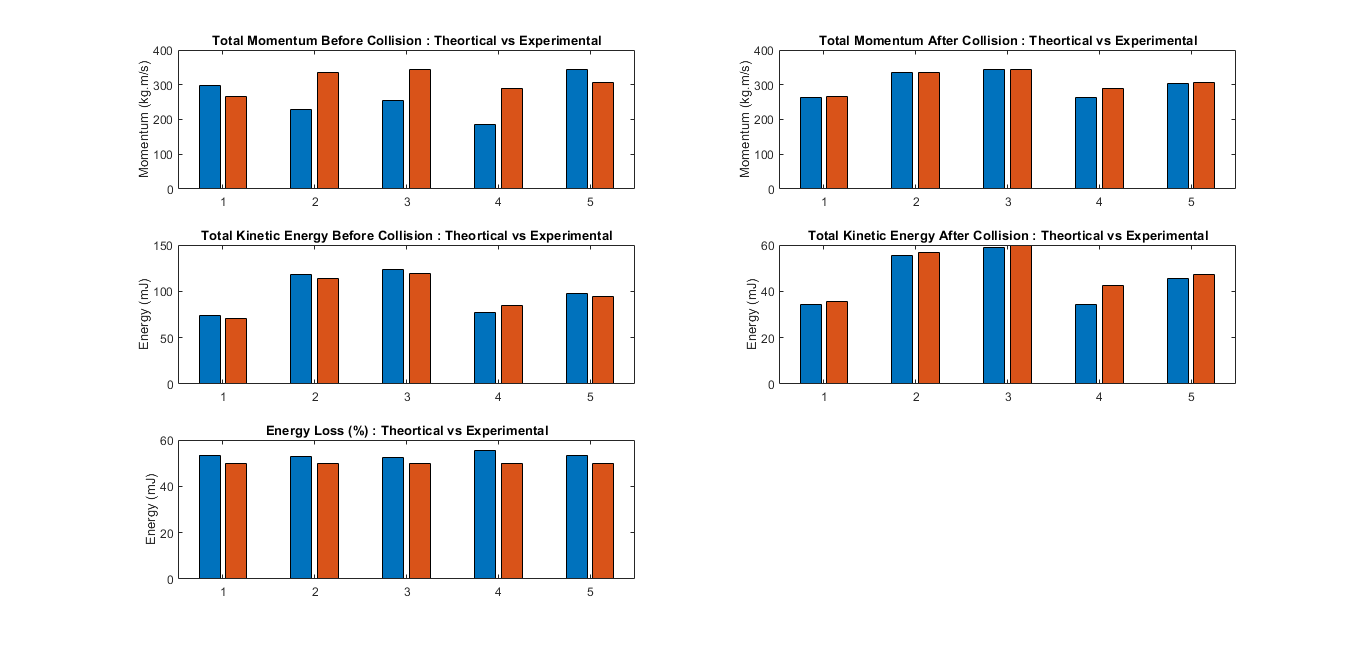
\includegraphics[width=\textwidth]{figures/Exp3.png}
    \caption{In-Elastic Collision with $m_1 = m_2$}
    \label{fig:yx}
\end{figure}
\newpage
\begin{figure}[h!]
    \centering
    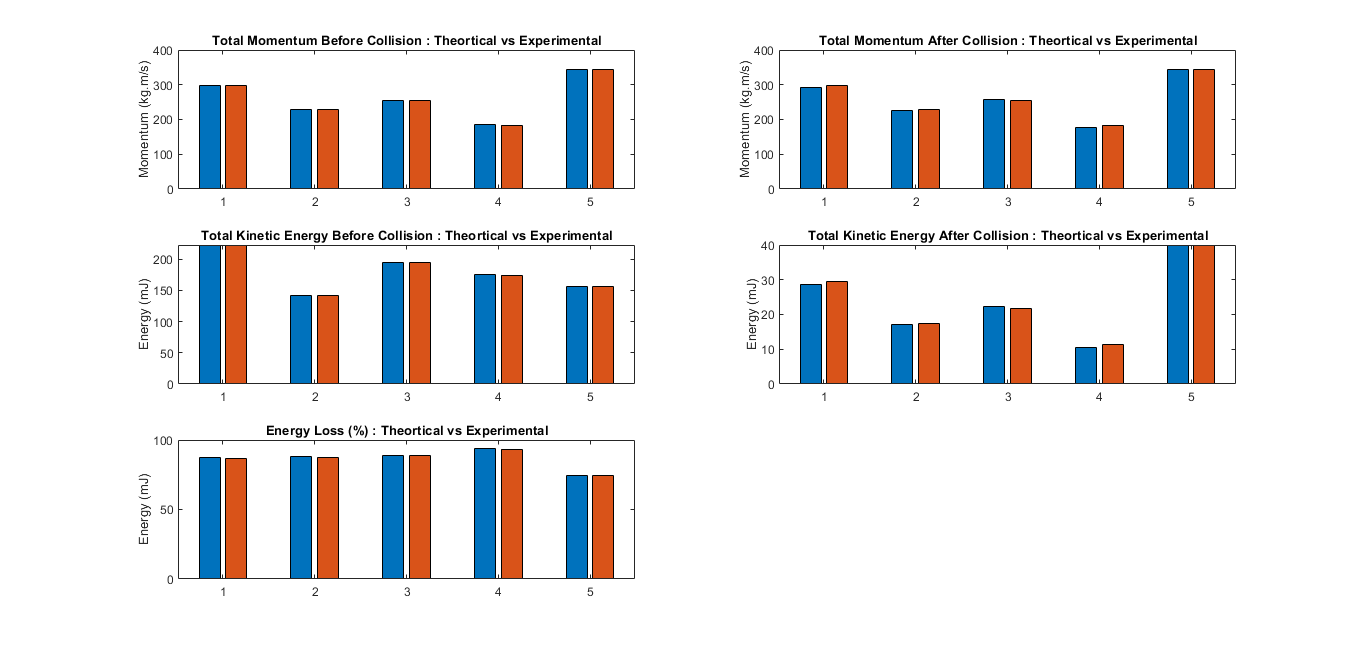
\includegraphics[width=\textwidth]{figures/Exp4.png}
    \caption{In-Elastic Collision with $m_1 \neq m_2$}
    \label{fig:yx}
\end{figure}

\section{Discussion \& Conclusion}

In both elastic and in-elastic, the experiment values agreed with the theoretical values up to a great extent when $m1\neq m2$. This is because in reality we didn't use equal masses. Moreover, elastic collisions don't occur in nature unless they are atomic in nature.



\section{MATLAB Script}
\lstinputlisting{matlabCodes/Experiment5.m}




\chapter{Equation of motion for angular motion}

Date: 29/10/2020

\section{Aim}
The aim of this experiment is to determine the angular acceleration and angular displacement for rotational motion using curve fitting in MATLAB. We also aim to derive equations of motion for rotational motion.


\section{Background Theory}

Rotational motion has similar characteristics to linear motion that is known as transnational motion. Rotational bodies have a moment of inertia similar to mass. The kinematics of rotational motion describes the relationships among rotation angle, angular velocity, angular displacement, angular acceleration, and time. Similar to linear motion equations, rotational motion equations can be written from the table provided in the manual. 
For linear equation $$ v=v_0 +at$$ Rotational can be written as following. In rotational $a = \alpha$ and $ a= r \alpha$ as angular acceleration is constant. $v=r \omega$ for rotational. Therefore 
$$ r \omega = r \omega_0 + r\alpha t $$ 
$$ \omega=\omega_0 + \alpha t$$
For linear equation $$ S= S_0 + v_i t + \frac{1}{2} a t^2$$. In rotational motion $S=\theta$ , $v=\omega$ , $a=\alpha$. Therefore 
$$\theta = \theta_0 + \omega_i t + \frac{1}{2} \alpha t^2 $$

% This section is meant to explain the theoretical background of the experiment whose report you are writing. Theoretical background \ref{eq:line} does not mean historical background. Be precise to, ONLY include scientific background.
% Table generated by Excel2LaTeX from sheet 'Sheet1'



% \begin{equation}
%     y = mx + c 
%     \label{eq:line}
% \end{equation}

% \begin{equation} \label{eq1}
% \begin{split}
% A & = \frac{\pi r^2}{2} \\
%  & = \frac{1}{2} \pi r^2
% \end{split}
% \end{equation}

\section{Description of Setup}
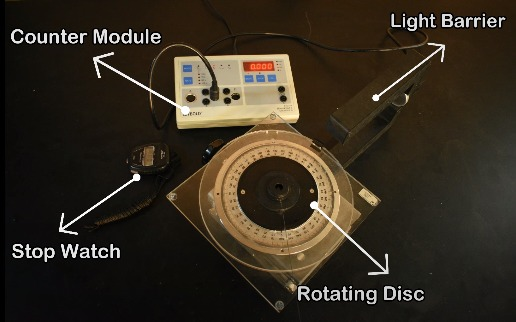
\includegraphics[width=10cm, height=7cm]{figures/exp6fig.jpeg} \\
Using the setup above, a light barrier is attached to the lab bench using a table clamp to place a rotating disk. The counter module and light barrier record the time when the flag interrupts the barrier. The stopwatch is used to record the time from rotation to when the main platter is detected. A pulley and thread help rotate the disk at constant acceleration. 
% Sketch and explain the experimental setup. The explanation should try to cover these pointers:  table \ref{tab:addlabel}
% \begin{enumerate}
%     \item What is the purpose of individual items in the setup?
%     \item If any equipment is taking measurements, what is it reading and how is it being read?
% \end{enumerate}

% Be precise to, ONLY include scientific description.

\section{Method / Procedure}

The experiment was set up and the disk was rotated at an angle of 90' and stopwatch was started when disk was released. The stop watch was stopped when the flag was detected by motion detector. 
The time measured by stopwatch and light gate at that angle was noted and repeated four times. 
The process was repeated five times by rotating disk at an angle of 120, 150, 180, 210, 240, 270 and 300'.
The respected data was recorded. 


% Highlight the following aspects of the experiment conducted 
% \begin{enumerate}
%     \item What method did you use to perform the experiment?
%     \item What adjustments were made, if any? 
%     \item What data was collected?
%     \item How was it collected?
%     \item Were any calibrations made and what were they?
% \end{enumerate}

% Be precise to, ONLY include scientific background.

\section{Data}

The type B uncertainty associated with the angle $\theta$ is 0.04 degrees. The type B associated uncertainty with the time T is $0.003$s

\begin{center}
\begin{tabular}{|l|l|l|}
\hline
\textbf{s.No} & \textbf{Angle} & \textbf{angle (°)} \\ \hline
1             & A1             & 90                 \\ \hline
2             & A2             & 120                \\ \hline
3             & A3             & 150                \\ \hline
4             & A4             & 180                \\ \hline
5             & A5             & 210                \\ \hline
6             & A6             & 240                \\ \hline
7             & A7             & 270                \\ \hline
8             & A8             & 300                \\ \hline
\end{tabular}
\end{center}

\begin{center}
  

\begin{tabular}{|l|l|l|l|l|l|l|l|l|}
\hline
\multicolumn{9}{|c|}{\textbf{Time period from Start to Cut}} \\ \hline
\textbf{s.No} &
  \textbf{T\_A1 (s)} &
  \textbf{T\_A2 (s)} &
  \textbf{T\_A3 (s)} &
  \textbf{T\_A4 (s)} &
  \textbf{T\_A5 (s)} &
  \textbf{T\_A6 (s)} &
  \textbf{T\_A7 (s)} &
  \textbf{T\_A8 (s)} \\ \hline
1  & 1.94  & 2.31  & 2.59 & 2.66 & 2.88 & 3.25 & 3.35 & 3.47 \\ \hline
2  & 1.93  & 2.31  & 2.65 & 3    & 3.03 & 2.84 & 3.35 & 3.35 \\ \hline
3  & 1.81  & 2.41  & 2.75 & 2.62 & 2.9  & 2.65 & 3.22 & 3.46 \\ \hline
4  & 2.03  & 2.34  & 2.84 & 2.69 & 2.75 & 3.19 & 3.34 & 3.42 \\ \hline
5  & 2.09  & 2.63  & 2.63 & 2.59 & 2.87 & 3.04 & 3.28 & 3.41 \\ \hline
\end{tabular}
\end{center}

\begin{center}
\begin{tabular}{|l|l|l|l|l|l|l|l|l|}
\hline
\multicolumn{9}{|c|}{\textbf{Time period from Start to Cut}} \\ \hline
\textbf{s.No} &
  \textbf{T\_A1 (s)} &
  \textbf{T\_A2 (s)} &
  \textbf{T\_A3 (s)} &
  \textbf{T\_A4 (s)} &
  \textbf{T\_A5 (s)} &
  \textbf{T\_A6 (s)} &
  \textbf{T\_A7 (s)} &
  \textbf{T\_A8 (s)} \\ \hline
1  & 1.94  & 2.31  & 2.59 & 2.66 & 2.88 & 3.25 & 3.35 & 3.47 \\ \hline
2  & 1.93  & 2.31  & 2.65 & 3    & 3.03 & 2.84 & 3.35 & 3.35 \\ \hline
3  & 1.81  & 2.41  & 2.75 & 2.62 & 2.9  & 2.65 & 3.22 & 3.46 \\ \hline
4  & 2.03  & 2.34  & 2.84 & 2.69 & 2.75 & 3.19 & 3.34 & 3.42 \\ \hline
5  & 2.09  & 2.63  & 2.63 & 2.59 & 2.87 & 3.04 & 3.28 & 3.41 \\ \hline
\end{tabular}
\end{center}

\begin{center}
\begin{tabular}{|l|l|l|}
\hline
Angle(rad) & Light Flag(s) & Stopwatch(s) \\ \hline
1.5707963  & 0.100081      & 1.96         \\ \hline
2.0943951  & 0.087436      & 2.4          \\ \hline
2.6179939  & 0.078868      & 2.692        \\ \hline
3.1415927  & 0.072822      & 2.712        \\ \hline
3.6651914  & 0.067409      & 2.886        \\ \hline
4.1887902  & 0.060538      & 2.994        \\ \hline
4.712389   & 0.060429      & 3.307        \\ \hline
5.2359878  & 0.056155      & 3.42167      \\ \hline
\end{tabular}
\end{center}

\newpage
\begin{figure}[h!]
    \centering
    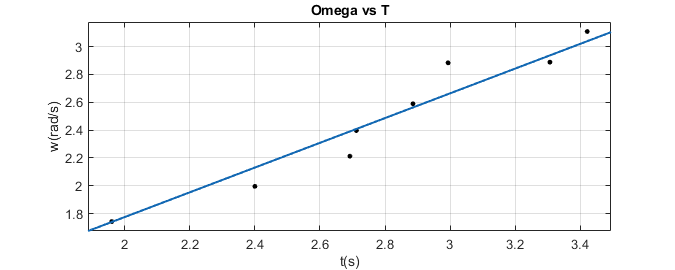
\includegraphics[width=\textwidth]{figures/omega_vs_t.png}
    \caption{Graph of $\omega$ vs t}
    \label{fig:yx}
\end{figure}
$$ \omega_f = \alpha t$$
$$ \alpha = 0.888 rad/s^2 $$


\begin{figure}[h!]
    \centering
    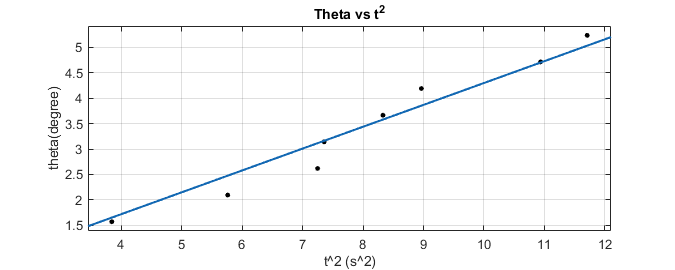
\includegraphics[width=\textwidth]{figures/theta_vs_t2.png}
    \caption{Graph of $\theta$ vs $t^2$}
    \label{fig:yx}
\end{figure}
$$ \theta = \alpha t^2$$
$$ \alpha = 0.430 rad/s^2 $$


\section{Data Analysis}

\newpage
\begin{figure}[h!]
    \centering
    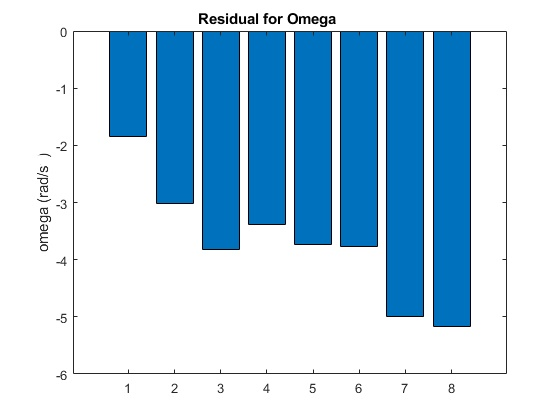
\includegraphics[width=\textwidth]{figures/res_omega.jpg}
    \caption{Residual plot for omega}
    \label{fig:yx}
\end{figure}


\newpage
\begin{figure}[h!]
    \centering
    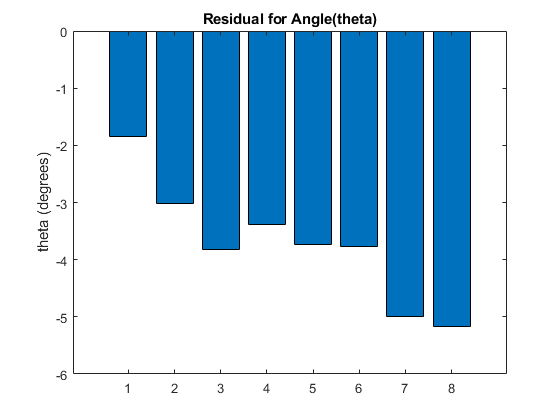
\includegraphics[width=\textwidth]{figures/res_theta.png}
    \caption{Residual plot for theta}
    \label{fig:yx}
\end{figure}


\section{Discussion \& Conclusion}

The graphs of $\omega$ vs t and $\theta$ vs $t^2$ are linear with an equal distribution of points on line as predicted by our hypothesis which verifies the equations of angular motion. There is a degree of uncertainty and error in the instruments while measuring time and angle, 0.04 for angle and 0.003 for time respectively. Reasons for points varying from the exact position on line include human error while measuring the time from stopwatch. Friction in the pulley, air resistance can also affect our experimental values. The degree of errors is increasing with increasing omega as seen in figure 6.3. 

% Summarize and discuss the experimental results, what do the results say about your hypothesis, if such a hypothesis was made for the experiment. Mention the uncertainty in the calculated quantity Be precise and only include scientific discussion.


\section{MATLAB Script}
\lstinputlisting{matlabCodes/Experiment6.m}




\chapter{Energy Conservation in Maxwell’s Wheel}

Date: 8/11/2020

\section{Aim}

The aim of this experiment is to understand the principle of conservation of energy and how it is distributed among the translational and rotational motion. We study the combination of rotational and transalational motion in a Maxwell's wheel




\section{Background Theory}

In transalational motion of an object, the entire object can be considered as a single point. All points of the object move in similar fashion and hence can be described from the same equation  of motion.  
However, rotational objects cannot be replaced by a single point as it is done in transalational motion.
Different points on the object are moving with different  speeds, depending on the distance from the axis of rotation. \\
The potential energy of the Maxwell's wheel is given by the expression,
\begin{equation}
    U =  mgh
\end{equation}
where m is the mass of the object and h is the maximum height . \\
The transalational kinetic energy of the Maxwell's wheel is given by the expression,
\begin{equation}
    KE =  \frac{1}{2}mv^2
\end{equation}
where m is the mass of the object and  v is the linear speed.\\
The rotational kinetic energy of the Maxwell's wheel is given by the expression,
\begin{equation}
    RE =  \frac{1}{2}I\omega^2
\end{equation}
where I is the moment of the Inertia and  $\omega$ is the angular speed.\\
As the wheel rotates, the change in the potential is equal to the sum of the transalational kinetic and rotational kinetic energy.
\begin{equation}
    \Delta U = KE + RE
\end{equation}
\begin{equation}
    mg\Delta h = \frac{1}{2}mv^2  + \frac{1}{2}I\omega^2
\end{equation}
where  $\Delta h$ is the height of the Maxwell's wheel from the surface of the table. \\
We can write $v = \omega r$, giving us the equation. 
\begin{equation}
    mg\Delta h = \frac{1}{2}mv^2  + \frac{1} { 2 r ^2}I v ^  2
\end{equation}
Re-arranging equation 7.6 and making $v^2$ as the subject gives us the following equation.
\begin{equation}
    v^2 = \frac{2mgr^2}{mr^2 + I} \Delta h
\end{equation}
\newpage
\section{Description of Setup}
\begin{figure}[h!]
    \centering
    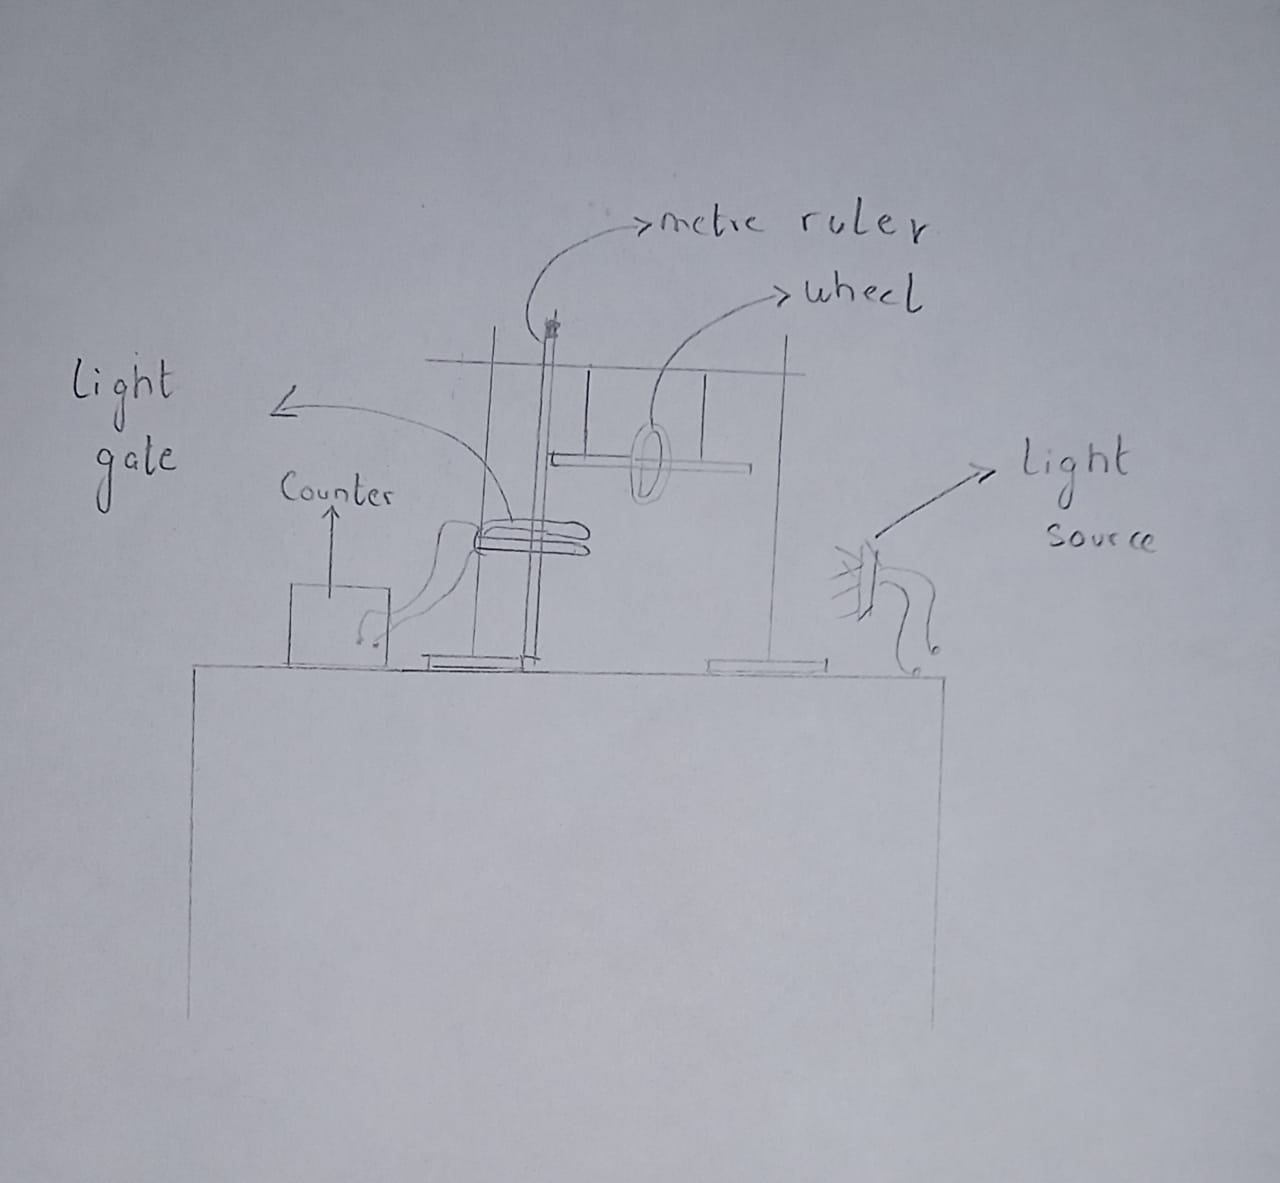
\includegraphics[width=\textwidth]{figures/Sktech.jpeg}
    \caption{Sketch of the experiment setup.}
    \label{fig:yx}
\end{figure}
Here the Light Gate and counter is used to measure translation speed v at given heights, the metre scale is used to measure the height of the Maxwell wheel $\Delta h$ with respect from the surface of the table.
\section{Method / Procedure}
The Maxwell's wheel is rotated up about its spindle such that the cord uniformly wounds about the spindle. When the wheel is released, it then falls as the chord unwinds. The speed of the translational of the wheel is calculated using the formula $ v = \frac{d}{t}$ where d is the diameter of the spindle and t is the time recorded by the counter. The height $\Delta h$ is adjusted by changing the position of the light gate. The above process is repeated 5 times for each $\Delta h$ and we chose 5 different values of the $\Delta h$.  The graph of $v^2$ vs $\Delta h$ and then slope of best fit is determined. The value of the best slope and the equation 7.7 is used to calculate the value of the moment of Inertia, I
\section{Data}
The type B uncertainty associated with the height h is $0.002m$ and the time is $0.0000003s$.  The mass of the object is $ m = 0.450 kg $ , the diameter of the wheel is  $ 0.13m$ and the diameter of the spindle is $ 0.003 m$

\begin{center}
\begin{tabular}{|l|l|l|l|l|}
\hline
\multicolumn{1}{|c|}{s.No} & \multicolumn{1}{c|}{$\Delta h(m)$} & \multicolumn{1}{c|}{Avg t(s)} & \multicolumn{1}{c|}{v (m/s)} & \multicolumn{1}{c|}{ $v^2 (m^2/s^2) $}\\ \hline
1                          & 0.44                                            & 0.0321104                     & 0.186855                     & 0.034914921                                                                           \\ \hline
2                          & 0.37                                            & 0.03222875                    & 0.186169                     & 0.034658964                                                                           \\ \hline
3                          & 0.3                                             & 0.032023333                   & 0.187363                     & 0.035105036                                                                           \\ \hline
4                          & 0.23                                            & 0.031566                      & 0.190078                     & 0.03612962                                                                            \\ \hline
5                          & 0.16                                            & 0.031749                      & 0.188982                     & 0.035714321                                                                           \\ \hline
\end{tabular}
\end{center}

\section{Data Analysis}

\begin{center}
\begin{adjustbox}{width=1\textwidth}
\begin{tabular}{|l|l|l|l|l|l|l|l|}
\hline
s.NO & TypeTimeA    & TypeBTime & TimeUncertainity & TimeVelocity    & HeightB     & TimeHeight      & Combined        \\ \hline
1    & 0.000324683  & 0.0000003 & 0.000325         & 0.0000001360356 & 0.000204124 & 0.0000156804345 & 0.0000156810245 \\ \hline
2    & 0.0000350323 & 0.0000003 & 0.000035         & 0.0000000128247 & 0.000204124 & 0.0000156804345 & 0.0000156804397 \\ \hline
3    & 0.0001901485 & 0.0000003 & 0.000190         & 0.0000000555547 & 0.000204124 & 0.0000156804345 & 0.0000156805329 \\ \hline
4    & 0.0001874448 & 0.0000003 & 0.000187         & 0.0000000417399 & 0.000204124 & 0.0000156804345 & 0.0000156804900 \\ \hline
5    & 0.0001901485 & 0.0000003 & 0.000190         & 0.0000000252239 & 0.000204124 & 0.0000156804345 & 0.0000156804548 \\ \hline
\end{tabular}
\end{adjustbox}
\end{center}

\begin{figure}[h!]
    \centering
    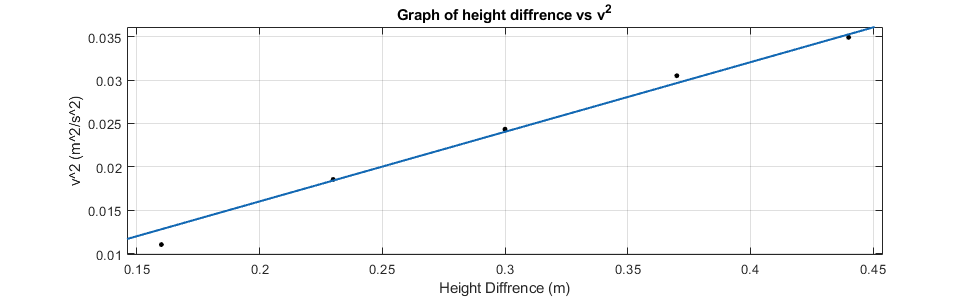
\includegraphics[width=\textwidth]{figures/AvgH_v2.png}
    \caption{Graph of y vs x}
    \label{fig:yx}
\end{figure}
\begin{equation}
    v^2 = 0.0814 \Delta h
\end{equation}
The gradient $ a = 0.0814 $

\begin{equation}
    gradient = \frac{2mgr^2}{mr^2 + I}  \Delta h
\end{equation}
Making the I,moment of inertia as a subject gives us the equation
\begin{equation}
    I  = \frac{2mgr^2 -amr^2}{a}
\end{equation}
where a is the gradient, m is the mass of object, g is the gravitational acceleration and r is the radius of the spindle. 
\begin{itemize}
    \item $ m = 0.450 kg $
    \item $ g = 9.80665 m/s^2 $
    \item $ r = 0.003 m$
\end{itemize}
Using the equation 7.8 and the above values we can calculate the value of I, the moment of Inertia 
$$ I  = \frac{2 \times 0.450 \times 9.80664 \times 0.003^2 -0.0814 \times 0.450 \times 0.003^2}{0.0814} = 0.97178 \times 10^{-3} kg m^2$$

\begin{figure}[h!]
    \centering
    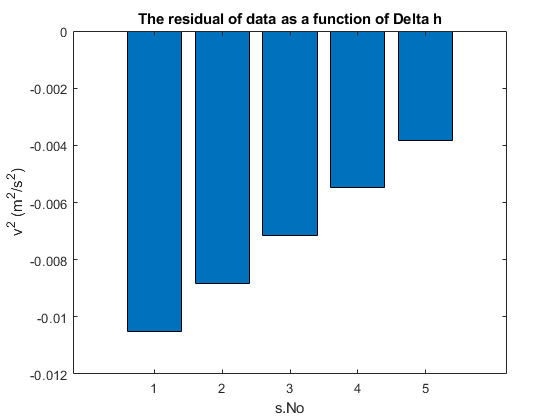
\includegraphics[width=\textwidth]{figures/residual_h.png}
    \caption{Residual of actual as a function of delta H}
    \label{fig:yx}
\end{figure}



\section{Discussion \& Conclusion}

The graph of $v^2$ vs $\Delta h$ is a linear which suggests a linear trend. Furthermore, the actual value of the Moment of Inertia I, $1.03 \times 10^-3 kg m^2$ is very close to the measured value of the Moment of Inertia, $0.9718 \times 10^-3 kg m^2 $ . The residual plot of the actual data as the function of $\Delta h$  shows a certain pattern which indicates the pattern of a systematic error. One of the possible sources of these systematic errors energy losses due to friction


\section{MATLAB Script}
\lstinputlisting{matlabCodes/Experiment7.m}




\chapter{Latent Heat of Vaporization of Liquid Nitrogen}

Date: 5/11/2020

\section{Aim}
The aim of this experiment is to understand latent heat of vaporization through liquid nitrogen and safe use of cryogens through a setup of circuits for heating and measurement of current and voltage through liquid nitrogen. 


\section{Background Theory}

Latent heat is defined as energy released or absorbed when a substance changes state. Latent heat absorbed when a solid changes to liquid is latent heat of fusion. Latent heat absorbed when a liquid changes to vapour, to break inter-molecular forces, is known as latent heat of vaporisation. It can be calculated using 
$$ L_v = \frac{\triangle Q}{\triangle m}$$ 
where Q is amount of energy and m is mass. 
Liquid Nitrogen is an odourless and a colourless fluid that starts to evaporate at room temperature


\section{Description of Setup}
\includegraphics[width=10cm, height=7cm]{figures/image.png} \\
Using the setup above, a resistor is attached to variac through an ammeter in series. Liquid Nitrogen is used in a Styrofoam cup to isolate it thermally to calculate latent heat. An electronic balance is used to measure the change in mass of nitrogen as it is heated.  


\section{Method / Procedure}
The apparatus was set up and liquid nitrogen was poured from a cryogenic container into the Styrofoam cup using gloves and safety goggles. The mass of the cup with resistor inside was measured and the mass lost is measured. Start the stopwatch timer and wait for 20 seconds. Note mass for every second for 30 seconds. Start the variac and heater which increases the rate of mass loss. The mass was recorded for every second for 30 seconds. The heating was then turned off for 30 seconds and mass recorded. The previous two steps are repeated one more time. At the end, the cup is removed and leftover liquid nitrogen is poured back.


\section{Data}
The type B uncertainty associated with time is 0.003s. The type B uncertainty associated with Mass is 0.03 g.  

\begin{center}
\begin{adjustbox}{width=1\textwidth}
\begin{tabular}{|l|l|l|l|l|l|l|l|l|}
\hline
     & \multicolumn{2}{c|}{heating off 1} & \multicolumn{2}{c|}{heating on 1} & \multicolumn{2}{c|}{heating off 2} & \multicolumn{2}{c|}{heating on 2} \\ \hline
s.No & time (s)      & Mass   (grams)     & time (s)     & Mass   (grams)     & time (s)      & Mass   (grams)     & time (s)     & Mass   (grams)     \\ \hline
1  & 20 & 90.2 & 50 & 88.8 & 80  & 83.6 & 110 & 82.6 \\ \hline
2  & 21 & 90.0 & 51 & 88.7 & 81  & 83.6 & 111 & 82.6 \\ \hline
3  & 22 & 89.9 & 52 & 88.7 & 82  & 83.6 & 112 & 82.6 \\ \hline
4  & 23 & 89.9 & 53 & 88.5 & 83  & 83.4 & 113 & 82.4 \\ \hline
5  & 24 & 89.8 & 54 & 88.3 & 84  & 83.4 & 114 & 82.2 \\ \hline
6  & 25 & 89.8 & 55 & 88.1 & 85  & 83.4 & 115 & 82.1 \\ \hline
7  & 26 & 89.8 & 56 & 88.0 & 86  & 83.4 & 116 & 81.9 \\ \hline
8  & 27 & 89.7 & 57 & 87.7 & 87  & 83.4 & 117 & 81.8 \\ \hline
9  & 28 & 89.6 & 58 & 87.7 & 88  & 83.4 & 118 & 81.6 \\ \hline
10 & 29 & 89.6 & 59 & 87.3 & 89  & 83.4 & 119 & 81.5 \\ \hline
11 & 30 & 89.5 & 60 & 87.2 & 90  & 83.3 & 120 & 81.2 \\ \hline
12 & 31 & 89.5 & 61 & 87.0 & 91  & 83.3 & 121 & 81.1 \\ \hline
13 & 32 & 89.5 & 62 & 86.8 & 92  & 83.2 & 122 & 81.0 \\ \hline
14 & 33 & 89.4 & 63 & 86.7 & 93  & 83.2 & 123 & 80.8 \\ \hline
15 & 34 & 89.4 & 64 & 86.5 & 94  & 83.2 & 124 & 80.6 \\ \hline
16 & 35 & 89.3 & 65 & 86.2 & 95  & 83.1 & 125 & 80.4 \\ \hline
17 & 36 & 89.3 & 66 & 86.2 & 96  & 83.1 & 126 & 80.2 \\ \hline
18 & 37 & 89.3 & 67 & 85.9 & 97  & 83.0 & 127 & 80.0 \\ \hline
19 & 38 & 89.2 & 68 & 85.8 & 98  & 83.0 & 128 & 80.0 \\ \hline
20 & 39 & 89.2 & 69 & 85.6 & 99  & 83.0 & 129 & 79.8 \\ \hline
21 & 40 & 89.2 & 70 & 85.4 & 100 & 83.0 & 130 & 79.6 \\ \hline
22 & 41 & 89.0 & 71 & 85.2 & 101 & 82.9 & 131 & 79.6 \\ \hline
23 & 42 & 89.0 & 72 & 85.2 & 102 & 82.9 & 132 & 79.4 \\ \hline
24 & 43 & 89.0 & 73 & 84.9 & 103 & 82.9 & 133 & 79.2 \\ \hline
25 & 44 & 89.0 & 74 & 84.8 & 104 & 82.8 & 134 & 79.0 \\ \hline
26 & 45 & 89.0 & 75 & 84.6 & 105 & 82.8 & 135 & 78.8 \\ \hline
27 & 46 & 88.9 & 76 & 84.5 & 106 & 82.8 & 136 & 78.8 \\ \hline
28 & 47 & 88.9 & 77 & 84.2 & 107 & 82.8 & 137 & 78.7 \\ \hline
29 & 48 & 88.8 & 78 & 84.1 & 108 & 82.8 & 138 & 78.5 \\ \hline
30 & 49 & 88.8 & 79 & 83.9 & 109 & 82.6 & 139 & 78.3 \\ \hline
\end{tabular}
\end{adjustbox}
\end{center}


% In this section, describe what data was recorded during the experiment. Mention which quantities are being measured, which quantity is independent, which is dependent and which are constants. Make this difference very explicit. Make sure to quantify and state the uncertainties in the recorded data. Be precise and primarily include numerical data.

\section{Data Analysis}

Rate of Change Mass at different times 
\begin{center}
\begin{tabular}{|l|l|}
\hline
Time            & Rate of Change of Mass (g/s) \\ \hline
Heating  Off 1  & -0.04349                     \\ \hline
Heating   On 1  & -0.1744                      \\ \hline
Heating   Off 2 & -0.03418                     \\ \hline
Heating   On 2  & -0.1562                      \\ \hline
\end{tabular}
\end{center}
The average rate of change in mass when heating is off is $-0.3884 g/s$ and the average of change in mass when heating is on is $ -0.1653 g/s$

% \includegraphics[width=8cm, height=7cm]{figures/on_1.png} \\
% \includegraphics[width=8cm, height=7cm]{figures/off_1.png} \\
% \includegraphics[width=10cm, height=7cm]{figures/on_2.png} \\
% \includegraphics[width=10cm, height=7cm]{figures/off_2.png} \\

% In this section, mention the calculations you perform, uncertainties transferred, and statistical analysis (residuals, errors, uncertainties in parameters fit etc.). Be precise and primarily include numerical data \ref{eq:line}.
\newpage
\begin{figure}[h!]
    \centering
    \includegraphics[width=\textwidth]{figures/TimeOff1_c.png}
    \caption{Heating Time Off 1}
    \label{fig:yx}
\end{figure}
The line of best fit : $ y = -0.04389x + 90.88$ \\
\newpage
\begin{figure}[h!]
    \centering
    \includegraphics[width=\textwidth]{figures/TimeOn1_c.png}
    \caption{Heating Time On 1}
    \label{fig:yx}
\end{figure}
The line of best fit : $ y = -0.01744x + 97.67$ \\
\newpage
\begin{figure}[h!]
    \centering
    \includegraphics[width=\textwidth]{figures/TimeOff2_c.png}
    \caption{Heating Time Off 2}
    \label{fig:yx}
\end{figure}
The line of best fit : $ y = -0.03418x + 86.12$ \\
\newpage
\begin{figure}[h!]
    \centering
    \includegraphics[width=\textwidth]{figures/TimeOn2_C.png}
    \caption{Heating Time On 2}
    \label{fig:yx}
\end{figure}
The line of best fit : $ y = -0.1562x + 99.99$ \\
\newpage
\begin{figure}[h!]
    \centering
    \includegraphics[width=\textwidth]{figures/Final.png}
    \caption{The graph of change in mass vs Time}
    \label{fig:yx}
\end{figure}

Rate of mass lost for electrical heating is calculated using 
\begin{equation}
    \frac{\triangle m}{\triangle t}_{Electric-heating} = \frac{\triangle m}{\triangle t}_{Electric-heating + Ambient-heat} - \frac{\triangle m}{\triangle t}_{Ambient-heat}
\end{equation} 
Therefore, rate of change in mass  is $-0.1265 g/s$. \\ 
Average Power dissipated is $29.323W$. \\
Using the equation we calculate Latent heat of vaporization. 
\begin{equation}
    L_v= \frac{VI}{\frac{\triangle m}{\triangle t}_{Electric-heating}}
\end{equation} 
Thus, our experimental value of $L_v$ is 
\begin{equation}
    L_v= \frac{29.323}{0.1265} = 231.8 J/g 
\end{equation} 
\newpage
\section{Discussion \& Conclusion}
The experimental value and theoretical value for Latent heat of vaporization have a huge difference. Thus, our hypothesis is not valid since experimental value for $L_v$ does not agree with theoretical. This is due to heat losses to the environment from liquid nitrogen as its boiling point is below room temperature which is why our values do not match. Heat losses could be minimized using high resolution apparatus that ensures the experiment is conducted in a controlled environment. The mass was also measured in grams using the electronic balance which has a higher uncertainty, but using an apparatus that could give smaller values of mass would give more accurate results. 
% Summarize and discuss the experimental results, what do the results say about your hypothesis, if such a hypothesis was made for the experiment. Mention the uncertainty in the calculated quantity Be precise and only include scientific discussion.

\section{MATLAB Script}
\lstinputlisting{matlabCodes/Experiment8.m}

% \section{MATLAB Script}
% \lstinputlisting{matlabCodes/test.m}




\chapter{Determining the Curie Temperature of Kanthal-D wire}

Date: 15/11/2020

\section{Aim}

The magnetic properties of materials depend upon the atomic and molecular arrangements within the material. These alignments also depend upon the temperature of the material. 
The aim of this experiment is to understand how temperature affects the magnetic properties of the Kanthal-D wire.


\section{Background Theory}

Both naturally-occurring and human-made materials have a range of magnetic properties. \textit{Ferromagnetic } materials posses an intrinsic magnetic field. Materials which acquire a magnetic field in the presence of external magnetic fields are called \textit{para-magnetic} materials. \textit{Diamagnetic} materials are those which are not affected by external magnetic fields. \\
The origin of magnetism in materials lies in the motion and configuration of electrons within an atom. These electrons constitute a current and hence produce a tiny magnetic for each atom. Each atom is called to make a magnetic dipole. The arrangement and orientation of these elementary dipoles determine the overall magnetic properties. If these magnetic dipoles are naturally aligned and kept in that configuration by the inter molecular forces, then the magnetic fields enforce each other and, as a result, the material gets an overall intrinsic magnetic field. These materials are called ferromagnetic materials.\\
Combinations of atoms are called \textit{magnetic domains}. Atoms within these magnetic domains are aligned in a certain direction on average. If these domains are randomly distributed it cancels the overall magnetic field of the material. In some materials, atoms in the domains, and thus the domain itself,can be made to align if an external magnetic field is applied. \\
In ferromagnets atoms in domains are aligned in a certain preferred direction and held in that place with the inter-molecular forces . In figure 1, boundaries between randomly aligned domains is shown in the absence and presence of a external magnetic fields.
\begin{figure}[h!]
    \centering
    \includegraphics[width=\textwidth]{figures/Domains.png}
    \caption{Graph of y vs x}
    \label{fig:yx}
\end{figure}\\
The thermal energy of atoms and molecules tends to the disturb the alignment of elementary magnets. As the temperature increases, the alignment is disturbed, and above a critical temperature, the \textit{Curie temperature } $T_C$, a ferromagnetic turns into a para-magnet. \\
The electrical energy supplied in $\Delta t$ time supplied by voltage $V$ and current $I$ can be calculated by the following equation 
\begin{equation}
    E_E = V I \Delta t    
\end{equation}
The energy $E_a$, absorbed in raising the temperature of the Kanthal wire is given in terms of specific heat of Kanthal wire and change in temperature,
\begin{equation}
    E_a = mc(T_C - T_0)
\end{equation}
The energy radiated $E_r$ ratiated from the wire is,
\begin{equation}
    E_r = \epsilon \sigma S ({T_c}^4 - {T_0}^4)\Delta t
\end{equation}
Combining equation 1 and 2, and re-arranging the terms gives us the following equation.
\begin{equation}
    -(mcT_o + \epsilon \sigma S {T_0}^4 \Delta t + V I \Delta t) + m c T_C + \epsilon\sigma S {T_C}^4 \Delta t = 0
\end{equation}

\section{Description of Setup}
\includegraphics[width=10cm, height=7cm]{figures/fig9exp.png} \\
The experiment is set up as above where the variac is attached to an ammeter, voltmeter and a control box. The kanthal-D wire is attached to a magnet with minimum area contact on a pole. A stopwatch is used to record the time taken to reach curie temperature. A digital ammeter and voltmeter is used to get accurate readings since the control box isn't precise. 


\section{Method / Procedure}
The kanthal-D wire is attached to the magnet in such a way that there is minimum area in contact. The control box is set up and green button is pressed to turn it on. The output voltage is set on 25.3 V on a variac and the current is measured using a digital ammeter. To turn off the control box the toggle switch is pressed. After the wire is cooled, we turn on the toggle switch and start the stopwatch. When the wire snaps away from the magnet, the stopwatch is stopped and we turn off the toggle switch. The time is recorded and the heating element is cooled. Four more readings at the same voltage are taken. The same procedure is repeated for nine different voltages on variac with 5 readings at every voltage.  

\section{Data}

The mass m of the Kanthal wire is $2.35 \pm 0.01$ gm,diameter is  $0.723\pm 0.002$ mm , length is $100 \pm 0.1 $cm, c specific heat capacity (c) is $460 J {Kg}^{-1}{K}^{-1}$ and the Emissivity ($\epsilon $) is 0.7 . $T_0$ the room temperature is taken as $25^\circ$ C.\\
The following data was recorded 
\begin{center}
\begin{tabular}{|c|c|c|c|}
\hline
\textbf{s.No} & \textbf{Voltage (V)} & \textbf{Current (A)} & \textbf{Avg\_t(s)} \\ \hline
1             & 25.3                 & 5.63                 & 14.29              \\ \hline
2             & 26.3                 & 5.87                 & 9.09               \\ \hline
3             & 27.2                 & 6.04                 & 8.76               \\ \hline
4             & 28.8                 & 6.39                 & 6.84               \\ \hline
5             & 29.3                 & 6.57                 & 5.74               \\ \hline
6             & 31.5                 & 6.95                 & 4.98               \\ \hline
7             & 33.2                 & 7.31                 & 4.20               \\ \hline
\end{tabular}
\end{center}

\section{Data Analysis}

Solving the the degree 4 polynomial equation gives us the value of the Curie Temperature $T_C$ for value of Voltage and Current.  
\begin{center}
\begin{tabular}{|c|l|}
\hline
\textbf{s.No} & Curie Temperature (Tc) / K \\ \hline
1             & 999.595                     \\ \hline
2             & 959.303                     \\ \hline
3             & 974.734                     \\ \hline
4             & 967.115                     \\ \hline
5             & 943.795                     \\ \hline
6             & 958.587                     \\ \hline
7             & 953.408                     \\ \hline
\end{tabular}
\end{center}
The average value of the Curie Temperature $T_C$ is $692.220^\circ C$. The type A uncertainty in the value of the Curie Temperature is $6.820^\circ C$. The final value is $ 692.220 \pm 6.820 ^\circ C$

\section{Discussion \& Conclusion}

The expected value of the Curie Temperature for the Kanthal-D wire is $600 ^\circ $ C whereas the calculated value is $692.220^\circ C$. One of the reasons for this huge difference is the environmental losses. The long wire radiates more heat since the room is open and room temperature is not maintained. Furthermore, the time that is being recorded is very small and since its being recorded by a stopwatch there is human reaction time. Instead of using a stopwatch, record the motion by a video camera and then playback frame by frame to know the exact moment the wire becomes detached. The experiment should be carried out in a close environment. 



\section{MATLAB Script}
\lstinputlisting{matlabCodes/Experiment9.m}




\chapter{Determining the coefficient of convective heat transfer}

Date: 20/10/2020

\section{Aim}
The aim of this experiment is to measure the change of temperature of a body as heat flows from it to the surrounding through convective losses where the concept of heat is the flow of thermal energy through conduction, convection, radiation.


\section{Background Theory}
Heat is transferred through conduction, convection and radiation. Conduction is the process whereby heat energy is transferred across a medium. There are materials which are good or poor conductors of heat just like there are materials which are good or bad conductors of electricity. Thus, thermal conduction is the transfer of energy by microscopic collisions of particles and movement of electrons within a body. The equation under thermal equilibrium is as following: 
$$P= \frac{dQ}{dt} = -kA \frac{T_2 - T_1}{L} $$ where P represents power transmitted, A represents area and $T_2 - T_1$ is temperature difference and L represents length. 
Specific heat capacity is defined as amount of energy required per unit mass to raise temperature by one unit. It is given by $$Q=mc \triangle T $$. When heat is lost by object with time then it can be calculated by differentiating the above formula: 
$$\frac{dQ}{dt} = -mc \frac{dT(t)}{dt} $$.

Thermal convection occurs when a liquid comes in contact with an object whose temperature is higher than that of it. When the less energetic molecules of the air encounter the fast vibrating molecules of the hotter object, they pick up some energy off the molecules of the hot surface. At the interface of the object and the air the process is exactly similar to conduction. But the temperature of the air soon rises at the surface causing them to be less dense. The molecules have more energy and the hot air rises. These molecules then transfer the thermal energy to neighboring molecules through collisions conduction as well as through the bulk flow of air convection. In practice, both of these modes of heat transfer go on, hands in hand. When the molecules cool down they become dense and sink and when are hot they become less dense and rise. 

For small temperature difference between a body and its surrounding, the rate of cooling of the body is directly proportional to the temperature difference and the surface area exposed. 

$$\frac{dQ}{dt}  (q – q_s)$$ where q and $q_s$ are temperature corresponding to object and surroundings.

Newton’s law of cooling concerns the process of thermal conduction through convection is mathematically stated as

$$\frac{dQ_{conv}}{dt} = hA(T_2-T_1)$$

When an amount Q heat is provided to cylindrical rod of a certain material to raise its temperature by an amount $\triangle T$. When the rod cools down through convection in air currents the same amount of energy is lost with time to convection. This heat loss is : 
 $$hA(T(t)-T_0) = \frac{dQ}{dt}=-mc \frac{dT(t)}{dt}$$ where T is temperature of rod. $T_0$ is temperature of surrounding, m is mass, A is area of convection and h is coefficient of heat transfer.  


\section{Description of Setup}
\includegraphics[width=10cm, height=7cm]{figures/fig10.png} \\

The experiment is set up as above where the cylinder is placed inside the cavity to provide a closed environment and a thermocouple is used to measure voltage against the temperature and is inputted into the CASSY software to record readings.Other equipment includes heating machine, graphite powder, weighing machine, temperature gun, and Vernier calipers. 

\section{Method / Procedure}

First the mass is measured using weighing machine, the length and diameter of the cylinders are measured using vernier calipers. Then the cylinder is placed inside the steel box on the hot plate. Then it is covered with graphite powder and heated up to 350 $^{\circ} C$  for 45 minutes.  After heating we attach a thermocouple to the heated cylinder and transfer the cylinder into the cavity with the fan off.One thermocouple is attached to the cylindrical cavity to measure the temperature of the air in the cylinder. Second thermocouple is attached to the heated cylinder through a clip.  Then CASSY software is opened and readings are recorded. The cylinder is removed from the cavity and the thermocouple is attached to another cylinder. Then we transfer the cylinder into the cavity with the fan on. The data is recorded on CASSY software. 

% Highlight the following aspects of the experiment conducted 
% \begin{enumerate}
%     \item What method did you use to perform the experiment?
%     \item What adjustments were made, if any? 
%     \item What data was collected?
%     \item How was it collected?
%     \item Were any calibrations made and what were they?
% \end{enumerate}

% Be precise to, ONLY include scientific background.

\section{Data}
The type B uncertainty in the mass of the rod 1 and rod 2 is $0.000003 grams$ , in the diameter of the rod 1 and rod 2 is $0.000002m$ and in the length of rod 1 and rod 2 is $0.00002m$. 

\begin{center}

\begin{tabular}{|l|l|l|}
\hline
\textbf{}                                               & \textbf{Rod 1} & \textbf{Rod 2} \\ \hline
\textbf{Mass (grams)}                                   & 114.47         & 114.45         \\ \hline
\textbf{Length (mm)}                                    & 24.95          & 25.23          \\ \hline
\textbf{Diameter  (mm)}                                 & 78.53          & 78.42          \\ \hline
\textbf{Specific Heat Capacity of Aluminium (J/(kg*K))} & 887            & 887            \\ \hline
\end{tabular}
\end{center}

\section{Data Analysis}
\begin{equation}
    hA(T(t) - T_0 ) = -mc \frac{dT(t)}{dt}
\end{equation}

\begin{equation}
    hA = \frac{-mc}{T(t) - T_0} \frac{dT(t)}{dt}
\end{equation}

\begin{equation}
   c+ hAt = -mc \times ln (T(t) - T_0)
\end{equation}

\begin{equation}
   c = -mcln (X_0)
\end{equation}

\begin{equation}
    -mcln (X_0)+ hAt = -mc \times ln (X(t))
\end{equation}

\begin{equation}
    -mcln (X_0)+ hAt = -mcln (X(t))
\end{equation}

\begin{equation}
   - hAt = mcln (X(t))  -mcln (X_0)
\end{equation}


\begin{equation}
    X(t) = X_0e^({\frac{-hAt}{mc}})
\end{equation}
\begin{center}
    
Units of h =$ \frac{W}{m^2K} $


\end{center}
\begin{center}
\begin{tabular}{|l|l|l|}
\hline
\textbf{}                                      & \textbf{Rod 1} & \textbf{Rod 2} \\ \hline
\textbf{Mass (grams)}                          & 114.4700       & 114.4500       \\ \hline
\textbf{Mass (kg)}                             & 0.1145         & 0.1145         \\ \hline
\textbf{Length (mm)}                           & 24.9500        & 25.2300        \\ \hline
\textbf{Length (m)}                            & 0.0250         & 0.0252         \\ \hline
\textbf{Diameter  (mm)}                        & 78.5300        & 78.4200        \\ \hline
\textbf{Diameter (m)}                          & 0.0785         & 0.0784         \\ \hline
\textbf{Surface Area }   & 0.0062         & 0.0062         \\ \hline
\end{tabular}
\end{center}

\newpage
\begin{figure}[h!]
    \centering
    \includegraphics[width=\textwidth]{figures/Subplots.png}
    \caption{Graph of Temperature vs Time}
    \label{fig:yx}
\end{figure}
\begin{center}
    Value of h without fan = $ 28.667 \frac{W}{m^2K} $
\end{center}
\begin{center}
    Value of h with fan = $ 40.1610 \frac{W}{m^2K} $
\end{center}
\section{Discussion \& Conclusion}

As expected as value of h with fan  $ 40.1610 \frac{W}{m^2K} $ is greater than h without fan $ 28.667 \frac{W}{m^2K} $. In the residual graph, there is an irregular pattern which indicates the presence of random error. The major source of this error is the heat loss to the environment. The Newton's Law of cooling is limited because the difference in temperature between the body and surroundings must be small. Another major limitation of Newton’s law of cooling is that the temperature of surroundings must remain constant during the cooling of the body.


\section{MATLAB Script}
\lstinputlisting{matlabCodes/Experiment10.m}




\chapter{Rotational Motion and Frictional Losses}

Date: 29/11/2020

\section{Aim}

The aim of this experiment is to understand energy losses due to frictional. We will study the relationship between frictional losses in 
a pulley and mass of the object.
    
%An aim is a short description of what you are about to do in the experiment. It usually answers the questions like, 
%\begin{enumerate}
 %   \item What are you plan on doing?
 %  \item How are you doing it?
  %  \item Why are you doing it?
%\end{enumerate}


\section{Background Theory}

%This section is meant to explain the theoretical background of the experiment whose report you are writing. Theoretical background does not mean historical background. Be precise to, ONLY include scientific background.

Consider the provided circular disks (rigid bodies) to be made up of small infinitesimal particles of masses $m_1,m_2,m_3, \cdots,m_n$. Their placement may be defined with the position vectors $\vec{r_1},\vec{r_2},\cdots.\vec{r_n}$ and when rotating, their instantaneous velocities may be defined as
$\vec{v_1},\vec{v_2},\vec{v_3} ,\cdot,\vec{v_n}$.
The angular momentum of a particle given is by
\begin{equation}
    \label{eq1}
    \vec{J_i} = m \vec{v_i} \times \vec{r_i}
\end{equation}
For a particle rotating with angular velocity 
$ \omega$ about z axis, we can say that
\begin{equation}
    \label{eq2}
    v_i = r_i \omega_i
\end{equation}
We can then combine \ref{eq1} and \ref{eq2} to obtain the following equation
\begin{equation}
    \vec{J_i} = m\vec{r_i}\vec{\omega_i}
\end{equation}
Then the total angular momentum of the disk is simply the sum of the angular momentum of the individual particles making the disk.
\begin{equation}
    \vec{J} = \sum_i^n  m\vec{r_i}^2\vec{\omega_i}
\end{equation}
The quantity $\sum_i^n  m\vec{r_i}^2$ is known as moment of Inertia I. In this form , the angular momentum of the disc becomes
\begin{equation}
    J_z = \omega I
\end{equation}
We can write I in the similar form as transalational moment,
\begin{equation}
    I = \frac{1}{2} M R^2
\end{equation}
Rotational Kinetic energy is defined as 
\begin{equation}
    K = \frac{1}{2} I \omega ^2
\end{equation}
Moment of inertia of a particular body is defined with respect to a particular rotation axis and is different for a body when it is rotating about x, y or z axes.







\section{Description of Setup}
\newpage
\begin{figure}[h!]
   \centering
    \includegraphics[width=\textwidth]{figures/Apparatus11.png}
    \caption{Apparatus and the arrangement of the experimental setup.}
    \label{fig:yx}
\end{figure}
Here the base is used to hold the platters and pulleys, main platter is the object which is performing the Rotational motion, camera and metre are used in conjunction to measure the height of the hanging mass, step pulley is used to adjust the torque , super pulley is used to provide a smooth transition from Translation to Rotational Motion and the Thread ans Mass are used to execute Translation Motion and rotate the main platter.

%Sketch and explain the experimental setup. The explanation should try to cover these pointers: 
%\begin{enumerate}
%   \item What is the purpose of individual items in the setup?
%   \item If any equipment is taking measurements, what is it reading and how is it being read?
%\end{enumerate}

%Be precise to, ONLY include scientific description.

\section{Method / Procedure}

%Highlight the following aspects of the experiment conducted 
%\begin{enumerate}
%   \item What method did you use to perform the experiment?
%   \item What adjustments were made, if any? 
%   \item What data was collected?
%    \item How was it collected?
%    \item Were any calibrations made and what were they?
%\end{enumerate}

%Be precise to, ONLY include scientific background.

In the given experimental setup, the thread is wrapped about the spindle as the wheel is spun. This lifts the mass tied to the other end of the thread by some distance, thereby storing potential energy in it. The disk is released, and the mass is let to oscillate for about five cycles, recording the height of the mass as a function of time.The same experiment using is for three other masses four masses. Then a graph of potential energy vs time is plotted in MATLAB for each particular value of Mass.

\section{Data}
The type B uncertainty in the height h is $0.001m$, in the time t is $0.003s$ and in the mass is $0.00003kg$.

\begin{center}
\begin{tabular}{|l|l|l|l|l|l|}
\hline
\multicolumn{6}{|c|}{\textbf{Mass (grams) = 23.3}} \\ \hline
\textbf{s.No} & \textbf{Time (s)} & \textbf{Max\_h (cm)} & \textbf{Min\_h (cm)} & \textbf{Diff\_h (cm)} & \textbf{P.E(J)} \\ \hline
0   & 0       & 68     & 12   & 56    & 0.1280009  \\ \hline
1   & 17.37   & 60     & 12   & 48    & 0.109715   \\ \hline
2   & 33.41   & 52     & 12   & 40    & 0.0914292  \\ \hline
3   & 48.09   & 45.5   & 12   & 33.5  & 0.076572   \\ \hline
4   & 62.37   & 40     & 12   & 28    & 0.0640004  \\ \hline
5   & 73.81   & 35.5   & 12   & 23.5  & 0.0537147  \\ \hline
\end{tabular}
\end{center}
\begin{center}
\begin{tabular}{|l|l|l|l|l|l|}
\hline
\multicolumn{6}{|c|}{\textbf{Mass (grams) = 43.0}} \\ \hline
\textbf{s.No} & \textbf{Time (s)} & \textbf{Max\_h (cm)} & \textbf{Min\_h (cm)} & \textbf{Diff\_h (cm)} & \textbf{P.E(J)} \\ \hline
0   & 0       & 68     & 12   & 56     & 0.236225  \\ \hline
1   & 12.21   & 62.5   & 12   & 50.5   & 0.219352  \\ \hline
2   & 24.12   & 56.5   & 12   & 44.5   & 0.202478  \\ \hline
3   & 35.71   & 51.5   & 12   & 39.5   & 0.183496  \\ \hline
4   & 46.89   & 46.5   & 12   & 34.5   & 0.166623  \\ \hline
5   & 57.16   & 43     & 12   & 31     & 0.153968  \\ \hline
\end{tabular}
\end{center}
\begin{center}
\begin{tabular}{|l|l|l|l|l|l|}
\hline
\multicolumn{6}{|c|}{\textbf{Mass (grams) = 62.6}} \\ \hline
\textbf{s.No} & \textbf{Time (s)} & \textbf{Max\_h (cm)} & \textbf{Min\_h (cm)} & \textbf{Diff\_h (cm)} & \textbf{P.E(J)} \\ \hline
0   & 0       & 68     & 12   & 56    & 0.3438994  \\ \hline
1   & 10.02   & 63.5   & 12   & 51.5  & 0.3162646  \\ \hline
2   & 20.27   & 58.5   & 12   & 46.5  & 0.2855593  \\ \hline
3   & 30.31   & 54     & 12   & 42    & 0.2579245  \\ \hline
4   & 39.43   & 50     & 12   & 38    & 0.2333603  \\ \hline
5   & 48.86   & 46.5   & 12   & 34.5  & 0.2118666  \\ \hline
\end{tabular}
\end{center}

\begin{center}
\begin{tabular}{|l|l|l|l|l|l|}
\hline
\multicolumn{6}{|c|}{\textbf{Mass (grams) = 82.2}} \\ \hline
\textbf{s.No} & \textbf{Time (s)} & \textbf{Max\_h (cm)} & \textbf{Min\_h (cm)} & \textbf{Diff\_h (cm)} & \textbf{P.E(J)} \\ \hline
0   & 0       & 68     & 12   & 56     & 0.451574  \\ \hline
1   & 9.2     & 64     & 12   & 52     & 0.419319  \\ \hline
2   & 18.45   & 60     & 12   & 48     & 0.387063  \\ \hline
3   & 27.09   & 55.5   & 12   & 43.5   & 0.350776  \\ \hline
4   & 35.54   & 51.5   & 12   & 39.5   & 0.318521  \\ \hline
5   & 43.62   & 48.5   & 12   & 36.5   & 0.294329  \\ \hline
\end{tabular}
\end{center}
%In this section, describe what data was recorded during the experiment. Mention which quantities are being measured, which quantity is independent, which is dependent and which are constants. Make this difference very explicit. Make sure to quantify and state the uncertainties in the recorded data. Be precise and primarily include numerical data.

\section{Data Analysis}

%In this section, mention the calculations you perform, uncertainties transferred, and statistical analysis (residuals, errors, uncertainties in parameters fit etc.). Be precise and primarily include numerical data.
Values obtained by curve Fitting of Potential Energy vs Time using the equation $ a \times e^{bt}$ are summarised in the following table.
\begin{center}
\begin{tabular}{|l|l|l|l|}
\hline
\multicolumn{4}{|c|}{Curve   Fitting Results} \\ \hline
s.No   & Mass(gram)   & a        & b (Frictional Loss Coefficient  )       \\ \hline
1      & 23.3         & 0.1305   & -0.01131   \\ \hline
2      & 43           & 0.2389   & -0.01034   \\ \hline
3      & 62.6         & 0.3467   & -0.00992   \\ \hline
4      & 82           & 0.4645   & -0.00986   \\ \hline
\end{tabular}
\end{center}

\begin{figure}[h!]
   \centering
    \includegraphics[width=1\textwidth]{figures/AllPlots.png}
    \caption{Graph of Height, Potential Energy vs Time and Residual Plots}
    \label{fig:yx}
\end{figure}



\newpage
\begin{figure}[h!]
   \centering
    \includegraphics[width=\textwidth]{figures/frictional.png}
    \caption{Graph of coefficient of Frictional Loss vs Mass}
    \label{fig:yx}
\end{figure}

\section{Discussion \& Conclusion}

%Summarize and discuss the experimental results, what do the results say about your hypothesis, if such a hypothesis was made for the experiment. Mention the uncertainty in the calculated quantity Be precise and only include scientific discussion.

The fit plot of Potential Energy vs Time is decreasing exponentially which is what we expected . Due to energy loss to friction, the maximum height decreased in each cycle and this turn meant that the potential energy decreased and we observed this in the plot. The graph of coefficient of frictional loss  vs mass has an increasing trend which means that more larger the mass , greater the energy loss. Sinusoidal pattern in the residual indicates the presence of random error. One way to improve these errors is to take more readings which can be done by taking more values of masses and recording maximum height for more cycles. 


\section{MATLAB Script}
\lstinputlisting{matlabCodes/Experiment11.m}




\chapter{Vibrations on Strings and Resonance}

Date: 12/04/2020

\section{Aim}

The aim of this experiment is to induce and observe standing waves on a string, identify where resonance occurs, to distinguishing linear from non-linear behaviour and compare experimental plots with mathematical relationships.

\section{Background Theory}

Wave is a disturbance or variation that transfers energy in a medium which provides the means for waves to propagate. Speed of a wave is given by 
\begin{equation}
v = \sqrt{\frac{T}{\mu}} 
\end{equation} 
A travelling wave oscillates in time and space. It is given by $Asin(kx-\omega t$. Where k is wave number related to wavelength of the wave and is given by 
\begin{equation}
    k=\frac{2\pi}{\lambda} \end{equation} 
and $\omega$ is angular frequency given by 
\begin{equation}
    \omega = 2\pi f = \frac{2\pi}{T}
\end{equation} Where f i frequency, T is time period of the wave. Therefore, speed of wave is given as \begin{equation}
    v=f \lambda = (\frac{\omega}{2\pi})(\frac{2\pi}{k}) = \frac{\omega}{k}
\end{equation} 
Interference is a phenomena that occurs when two waves meet travelling along same medium. There are two types, constructive and destructive. Constructive interference occurs when the crest meets crest or likewise for trough. A destructive interference happens when crest meets trough or the other way and leads to reduction of amplitude. 
Standing waves are formed by the interference of two traveling waves in opposite direction of same frequency and amplitude. Nodes are point where the total wave is zero at all times and anti-nodes are points that have maximum amplitudes. Distance between these two points is half wavelength. Harmonic is frequency where string vibrates with single antinode, called first harmonic. For higher harmonics frequency is given by \begin{equation}
    f_n = \frac{nv}{\lambda} = \frac{n}{\lambda} \sqrt{\frac{T}{\mu}}
\end{equation} and the frequency of nth harmonic is \begin{equation}
    f_n = \frac{n}{2L} \sqrt{\frac{T}{\mu}}
\end{equation}
When the string is loaded with beads, wave number is given as 
\begin{equation}
    k_n = \frac{2\pi}{\lambda_n} = \frac{n\pi}{(N+1)m}
\end{equation} U
sing previous equations we have \begin{equation}
    \frac{\omega_n}{v}=\frac{n\pi}{(N+1}m
\end{equation}
\begin{equation}
    \omega_n = 2\pi f_n=\frac{n\pi}{(N+1)m} \sqrt{\frac{T}{\mu}}
\end{equation}
\begin{equation}
    f_n = \frac{n}{2(N+1)m} \sqrt{\frac{T}{\mu}}
\end{equation}


\section{Description of Setup}
\newpage
\begin{figure}[h!]
   \centering
    \includegraphics[width=\textwidth]{figures/fig11.jpeg}
    \caption{Apparatus and the arrangement of the experimental setup.}
    \label{fig:yx}
\end{figure}
The experiment is set up as above with the string with and without beads, a signal generator, a speaker that produces waves and weight to create tension in string. 
% Sketch and explain the experimental setup. The explanation should try to cover these pointers:  table 
% \begin{enumerate}
%     \item What is the purpose of individual items in the setup?
%     \item If any equipment is taking measurements, what is it reading and how is it being read?
% \end{enumerate}

% Be precise to, ONLY include scientific description.

\section{Method / Procedure}
We first measure the diameter of the string using a micrometer, measure the length of the string using the meter rule. We also find the theoretical values to have a close frequency range for sweep frequency. We find the value of $\mu$ . Output leads of the signal generated to woofer is connected at 10V. Then we sweep the frequency of the signal generator and find the frequency at which standing waves appear. We do it for the first harmonic, second harmonic, third harmonic, fourth harmonic. We then repeat the same process for the loaded string, with beads, and measure the inter-bead distance first. We find the four harmonic frequencies in the same manner. We note down all harmonics and plot graph between frequency and number of the harmonics for both. 
% Highlight the following aspects of the experiment conducted 
% \begin{enumerate}
%     \item What method did you use to perform the experiment?
%     \item What adjustments were made, if any? 
%     \item What data was collected?
%     \item How was it collected?
%     \item Were any calibrations made and what were they?
% \end{enumerate}

% Be precise to, ONLY include scientific background.

\section{Data}
Type B uncertainty of diameter is 0.00002m and 0.002m for length and 0.002 for frequency. 

\begin{center}
\begin{tabular}{|c|c|c|c|c|}
\hline
\multicolumn{5}{|c|}{\textbf{un-loaded Steel String}} \\ \hline
       & h1        & h2        & h3        & h4       \\ \hline
S.no   & f1 (Hz)   & f2 (Hz)   & f3  (Hz)  & f4 (Hz)  \\ \hline
1      & 23.5      & 46.3      & 70.2      & 95.6     \\ \hline
2      & 24.14     & 50        & 73        & 93       \\ \hline
3      & 23.5      & 46        & 70.8      & 96       \\ \hline
\end{tabular}
\end{center}

\begin{center}
\begin{tabular}{|l|l|}
\hline
\multicolumn{2}{|c|}{\textbf{un-loaded Steel String}} \\ \hline
No. of Anti   Nodes      & Average Frequency(Hz)      \\ \hline
h1                       & 23.71333333                \\ \hline
h2                       & 47.43333333                \\ \hline
h3                       & 71.33333333                \\ \hline
h4                       & 94.86666667                \\ \hline
\end{tabular}
\end{center}

\begin{center}
\begin{tabular}{|c|c|c|c|c|}
\hline
\multicolumn{5}{|c|}{\textbf{Loaded Steel String}} \\ \hline
      & h1       & h2       & h3        & h4       \\ \hline
S.no  & f1 (Hz)  & f2 (Hz)  & f3  (Hz)  & f4 (Hz)  \\ \hline
1     & 13       & 26       & 35        & 44       \\ \hline
2     & 14       & 25       & 35        & 44       \\ \hline
3     & 12.7     & 24.5     & 35.6      & 44.5     \\ \hline
\end{tabular}
\end{center}


\begin{center}
\begin{tabular}{|l|l|}
\hline
\multicolumn{2}{|c|}{\textbf{Loaded Steel String}} \\ \hline
No. of Anti   Nodes     & Average Frequency(Hz)    \\ \hline
h1                      & 13.23333333              \\ \hline
h2                      & 25.16666667              \\ \hline
h3                      & 35.2                     \\ \hline
h4                      & 44.16666667              \\ \hline
\end{tabular}
\end{center}


% In this section, describe what data was recorded during the experiment. Mention which quantities are being measured, which quantity is independent, which is dependent and which are constants. Make this difference very explicit. Make sure to quantify and state the uncertainties in the recorded data. Be precise and primarily include numerical data.

\section{Data Analysis}
We have two equations for density and $\mu$ $$\rho = \frac{mass}{volume}$$ $$\mu =\frac{mass}{l}$$
We equate the two equations according to mass $$\rho * v = l *\mu$$ where v denotes volume and l denotes length. 
It is further divided into 
$$\rho * 2 \pi r^2 * l= l * \mu$$
We get our final equation as $$\mu = \rho * 2 \pi r^2 $$
Our values of tension T and $\mu $ are 11.9878 and 0.00314. 
Our theoretical values for harmonics are calculated using 
\begin{equation}
    f_n = \frac{n}{2L} \sqrt{\frac{T}{\mu}}
\end{equation}
 are as following: 
\begin{center}
\begin{tabular}{|l|l|}
\hline
\multicolumn{2}{|c|}{\textbf{un-loaded Steel String}} \\ \hline
No. of Anti   Nodes          & Frequency(Hz)          \\ \hline
h1                           & 16.96705               \\ \hline
h2                           & 33.9341                \\ \hline
h3                           & 50.90116               \\ \hline
h4                           & 67.86821               \\ \hline
\end{tabular}
\end{center}
\\
For loaded string we calculated harmonics using 
\begin{equation}
    f_n = \frac{n}{2(N+1)m} \sqrt{\frac{T}{\mu}}
\end{equation}
\begin{center}
\begin{tabular}{|l|l|}
\hline
\multicolumn{2}{|c|}{\textbf{Loaded Steel String}} \\ \hline
No. of Anti   Nodes         & Frequency(Hz)        \\ \hline
h1                          & 22.0571682           \\ \hline
h2                          & 44.11433639          \\ \hline
h3                          & 66.17150459          \\ \hline
h4                          & 88.22867278          \\ \hline
\end{tabular}
\end{center}

\newpage
\begin{figure}[h!]
   \centering
    \includegraphics[width=\textwidth]{figures/SubplotsExp12.png}
    \caption{Apparatus and the arrangement of the experimental setup.}
    \label{fig:yx}
\end{figure}

% In this section, mention the calculations you perform, uncertainties transferred, and statistical analysis (residuals, errors, uncertainties in parameters fit etc.). Be precise and primarily include numerical data \ref{eq:line}.

% \begin{figure}[h!]
%     \centering
%     \includegraphics[width=\textwidth]{figures/test.jpg}
%     \caption{Graph of y vs x}
%     \label{fig:yx}
% \end{figure}

\section{Discussion \& Conclusion}

We can see in the graph of Harmonics vs antinodes that there is a linear trend although, the value of harmonics does not double when the number of antinodes increase. Furthermore, we can see from both the residual plots that as the number of antinodes the error in the values of the harmonics also increase. This was expected because as the number of antinodes increase, the maximum amplitude decreases which in turn makes it difficult to observe.  We can reduce the random errors in this experiment by recording more values of harmonics for each antinodes. We can also vary the tension in string using different weights and then repeating the experiment for each value of Tension.

\section{MATLAB Script}
\lstinputlisting{matlabCodes/Experiment12.m}




\end{document}
